% Saberes básicos (LOMLOE) asociados a esta unidad
%
% Bloque B. La materia
%   - Teoría cinético-molecular: aplicación a observaciones sobre la materia
%     explicando la formación de mezclas y disoluciones — la unidad clasifica
%     mezclas homogéneas/heterogéneas, disoluciones, coloides y emulsiones a
%     partir del tamaño de partícula.
%   - Experimentos relacionados con los sistemas materiales: conocimiento y
%     descripción de sus propiedades, su composición y su clasificación —
%     se distinguen sustancias puras de mezclas y se caracteriza cada tipo
%     mediante propiedades como el punto de fusión o la concentración.
%   - Estructura atómica: desarrollo histórico de los modelos atómicos,
%     existencia, formación y propiedades de los isótopos y ordenación de los
%     elementos en la tabla periódica — se tratan los modelos de Dalton,
%     Thomson, Rutherford y Bohr, el número atómico, el número másico, los
%     isótopos y la organización en periodos y grupos.
%   - Principales compuestos químicos: su formación y sus propiedades físicas
%     y químicas, valoración de sus aplicaciones. Masa atómica y masa
%     molecular — se introduce el concepto de masa atómica al presentar
%     protones, neutrones e isótopos.
%   - Nomenclatura: formulando y nombrando sustancias simples, iones
%     monoatómicos y compuestos binarios mediante las reglas de nomenclatura
%     de la Iupac — se nombran y formulan compuestos binarios, hidróxidos e
%     iones monoatómicos sencillos.
%
% Bloque A. Las destrezas científicas básicas
%   - El lenguaje científico: unidades del Sistema Internacional — se usan de
%     forma consistente las unidades de masa y volumen (g, mL, g/L) al
%     calcular la concentración de las disoluciones.
%
% Esta unidad no desarrolla contenidos propios de los bloques C (la energía)
% ni D (la interacción), centrados en calor, electricidad, cinemática y
% fuerzas. Tampoco aborda el bloque E (el cambio), reservado a las
% reacciones químicas y su conservación de la masa, que se trabaja en otra
% unidad del curso.

\spacing{1.3}
\raggedbottom % pages with large figures end where the text ends (no stretched gaps between boxes)

\section{Pure substances and mixtures}

Look around you: water, air, a pencil, a sandwich\ldots{} Some of these things are made of \textbf{one} single substance, and others are made of \textbf{several} substances mixed together.

\begin{figure}[H]
    \centering
    % [FIGURA ORIGINAL] \includegraphics[width=\textwidth]{Unit_3/matter_classification}
    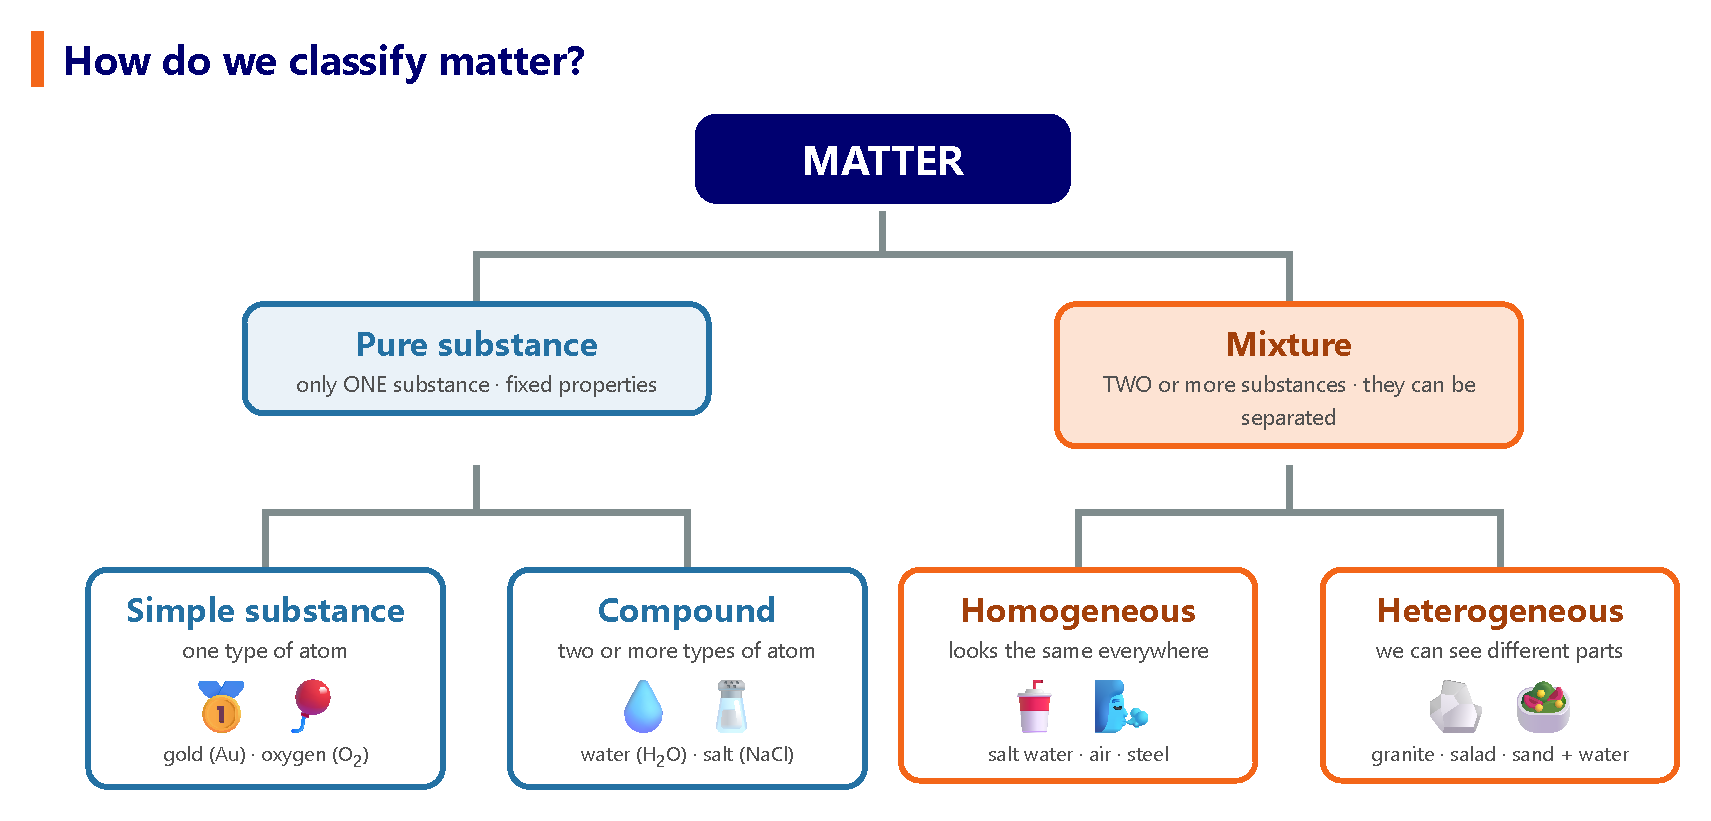
\includegraphics[width=\textwidth]{FigurasSVG/Unit_3_Diversity_of_Matter/pdf/matter_classification.pdf}
    \caption{Classification of matter.}
    \label{fig:u3_matter_classification}
\end{figure}

\begin{definition}[Pure substance]
    Matter made of \textbf{only one} substance. It has fixed, characteristic properties (for example, a fixed melting point). It can be a \textbf{simple substance} (one type of atom) or a \textbf{compound} (two or more types of atom).
\end{definition}

\begin{definition}[Mixture]
    Matter made of \textbf{two or more} substances. It is \textbf{homogeneous} if it looks the same everywhere (even with a microscope), and \textbf{heterogeneous} if we can see different parts.
\end{definition}

\begin{impt}
    \textbf{Pure substance or mixture?} Measure its melting point. Pure ice always melts at \qty{0}{\celsius}; different samples of butter (a mixture) melt at slightly different temperatures, because their composition is not fixed.
\end{impt}

\begin{exercise}
    Classify each example of matter according to its \textbf{appearance} (homogeneous or heterogeneous) and its \textbf{composition} (pure substance or mixture): sugar, salt water, granite, oxygen gas, milk.
    \begin{solu}
        \begin{center}
            \begin{tabular}{lll}
                \toprule
                \textbf{Matter} & \textbf{Appearance} & \textbf{Composition} \\
                \midrule
                Sugar & Homogeneous & Pure substance \\
                Salt water & Homogeneous & Mixture \\
                Granite & Heterogeneous & Mixture \\
                Oxygen gas & Homogeneous & Pure substance \\
                Milk & Looks homogeneous, but it is a colloid (heterogeneous) & Mixture \\
                \bottomrule
            \end{tabular}
        \end{center}
    \end{solu}
\end{exercise}

\begin{exercise}
    Say whether each example has a homogeneous or heterogeneous appearance: air, boiling water, smoke, yoghurt, sugar, crushed ice and lemon drink, milk and cocoa, paper with writing on it.
    \begin{solu}
        \textbf{Homogeneous}: air, sugar. \\
        \textbf{Heterogeneous}: boiling water (bubbles of gas in the liquid), smoke (solid particles in air), yoghurt, crushed ice and lemon drink, milk and cocoa, paper with writing on it.
    \end{solu}
\end{exercise}

\begin{exercise}
    Decide whether each system is a \textbf{pure substance} or a \textbf{mixture}, and justify your answer briefly: a) mineral water; b) oxygen gas (\ch{O2}); c) orange juice with pulp; d) sulphur powder (\ch{S}).
    \begin{solu}
        \begin{enumerate}[label=\alph*)]
            \item \textbf{Mixture}: water with several minerals dissolved in it.
            \item \textbf{Pure substance} (simple substance): only oxygen atoms.
            \item \textbf{Mixture} (heterogeneous): juice, water and visible pulp.
            \item \textbf{Pure substance} (simple substance): only sulphur atoms.
        \end{enumerate}
    \end{solu}
\end{exercise}

%----------------------------------------------------------------------------------------

\section{Homogeneous and heterogeneous mixtures}

Mixtures are classified by \textbf{what we can see}: can we tell their components apart just by looking at them, or not?

\subsection{Homogeneous mixtures}

\begin{definition}[Homogeneous mixture]
    A mixture whose components \textbf{cannot be distinguished with the naked eye}: it looks the same (uniform) in every part, and every sample of it has the same composition and the same properties.
\end{definition}

\begin{example}
    Some homogeneous mixtures we use every day:
    \begin{itemize}
        \item \textbf{Salt water} or \textbf{sugar dissolved in tea}: once the salt or the sugar has dissolved, we can no longer see it.
        \item \textbf{Air}: a mixture of nitrogen, oxygen, argon, carbon dioxide and other gases, but we cannot see any of them.
        \item \textbf{Mineral water} and \textbf{vinegar}: they look like a single clear liquid.
        \item \textbf{Steel} and \textbf{bronze}: metals mixed so well that they look like a single metal.
    \end{itemize}
\end{example}

The most important homogeneous mixtures are \textbf{solutions}, which we study in detail below.

\subsubsection{Solutions}

\begin{definition}[Solution]
    A \textbf{homogeneous} mixture of two or more substances. The \textbf{solvent} is the component in the largest amount; the \textbf{solute} (or solutes) is in a smaller amount.
\end{definition}

\begin{figure}[H]
    \centering
    % [FIGURA ORIGINAL] \includegraphics[width=\textwidth]{Unit_3/solution_parts}
    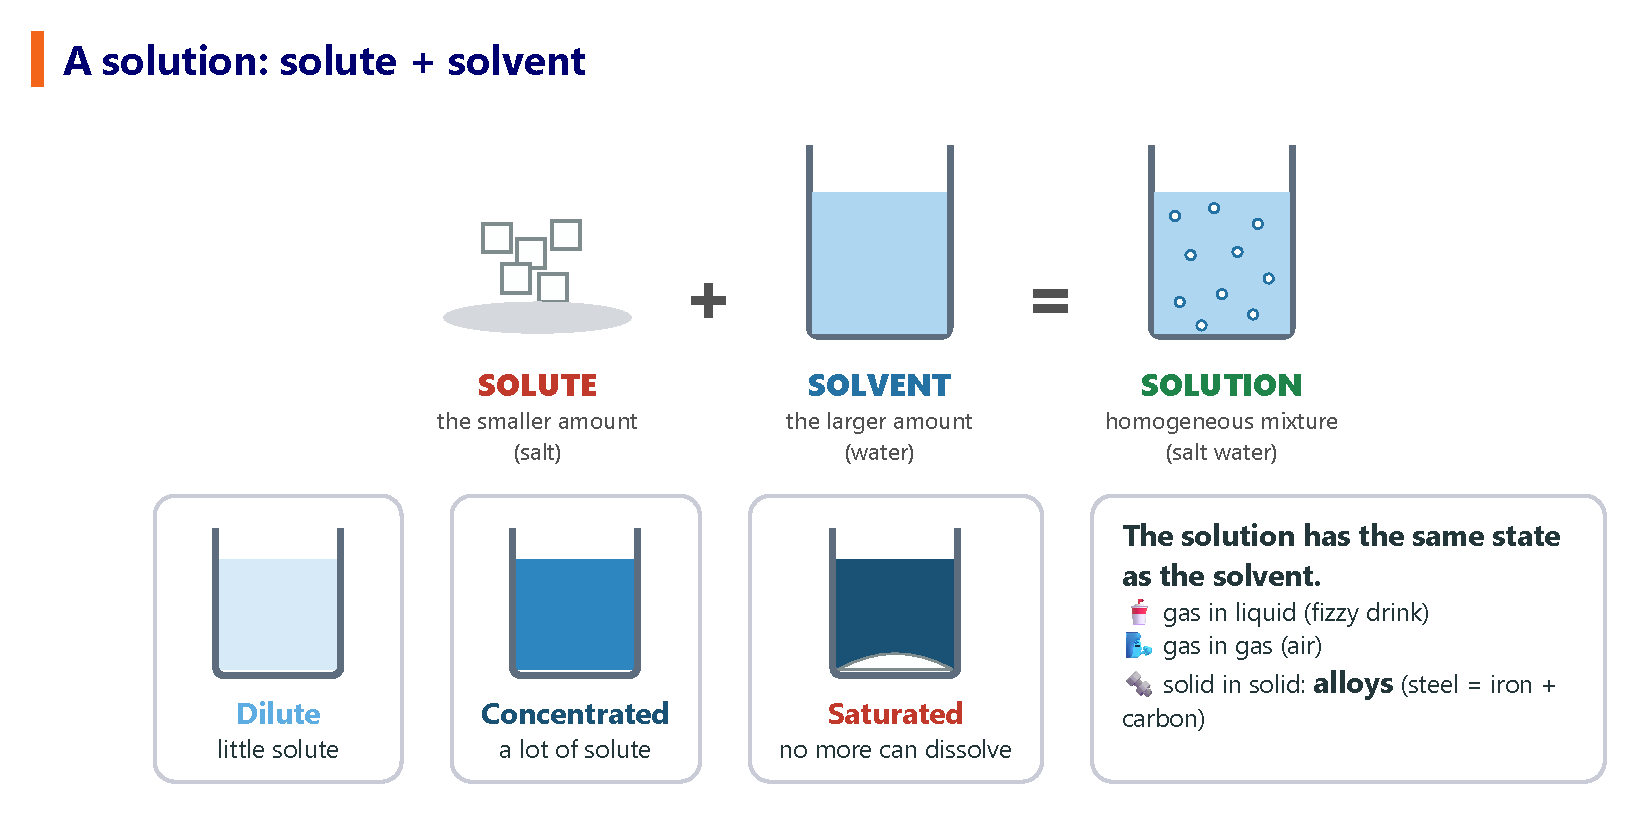
\includegraphics[width=\textwidth]{FigurasSVG/Unit_3_Diversity_of_Matter/pdf/solution_parts.pdf}
    \caption{The parts of a solution, and dilute, concentrated and saturated solutions.}
    \label{fig:u3_solution_parts}
\end{figure}

\begin{impt}
    A solution always has \textbf{one} solvent, but it can have \textbf{more than one solute}. For example:
    \begin{itemize}
        \item \textbf{Seawater}: the solvent is water, and the solutes are many different salts (sodium chloride, magnesium chloride, calcium sulfate\ldots).
        \item \textbf{A soft drink}: the solvent is water, and the solutes are sugar, carbon dioxide (the bubbles), colourings and flavourings.
        \item \textbf{Air}: the solvent is nitrogen, and the solutes are oxygen, argon, carbon dioxide and water vapour.
    \end{itemize}
\end{impt}

\begin{definition}[Alloy]
    A solid solution of two or more metals (or a metal and another element), made to improve the properties of the pure metal. Examples: steel (iron + carbon), bronze (copper + tin).
\end{definition}

\begin{exercise}
    For each mixture, indicate the physical state of the solute and of the solvent: air, sugar in water, steel, sparkling water, camomile tea.
    \begin{solu}
        \begin{center}
            \begin{tabular}{lll}
                \toprule
                \textbf{Mixture} & \textbf{Solute} & \textbf{Solvent} \\
                \midrule
                Air & Gas (oxygen, etc.) & Gas (nitrogen) \\
                Sugar in water & Solid & Liquid \\
                Steel & Solid (carbon) & Solid (iron) \\
                Sparkling water & Gas (\ch{CO2}) & Liquid \\
                Camomile tea & Solid/liquid & Liquid \\
                \bottomrule
            \end{tabular}
        \end{center}
    \end{solu}
\end{exercise}

\begin{exercise}
    A solution is made by mixing \qty{5}{\mL} of ethanol with \qty{45}{\mL} of water. Identify the solute and the solvent. Is this solution more or less concentrated than one made with \qty{20}{\mL} of ethanol and \qty{30}{\mL} of water?
    \begin{solu}
        Ethanol is in the smaller amount, so it is the \textbf{solute}; water is the \textbf{solvent}. \\
        The first solution has \qty{5}{\mL} of ethanol in \qty{50}{\mL}, and the second one \qty{20}{\mL} in \qty{50}{\mL}, so the first one is \textbf{more dilute} (less concentrated).
    \end{solu}
\end{exercise}

\begin{exercise}
    Give two examples of solutions found at home for each case: a) solid dissolved in liquid; b) liquid dissolved in liquid; c) gas dissolved in liquid.
    \begin{solu}
        \begin{enumerate}[label=\alph*)]
            \item Sugar in coffee; salt in soup.
            \item Vinegar (acetic acid in water); antifreeze in water.
            \item Sparkling water (\ch{CO2} in water); oxygen dissolved in the water of an aquarium.
        \end{enumerate}
    \end{solu}
\end{exercise}

\subsubsection{Concentration of solutions}

\begin{definition}[Concentration]
    The amount of solute dissolved in a given amount of solution.
\end{definition}

Before calculating any concentration, we must be very clear about what the \textbf{solution} is. The solution is \textbf{everything}: the solute (or solutes) \textbf{plus} the solvent.

\begin{figure}[H]
    \centering
    % [FIGURA ORIGINAL] \includegraphics[width=\textwidth]{Unit_3/solution_sum}
    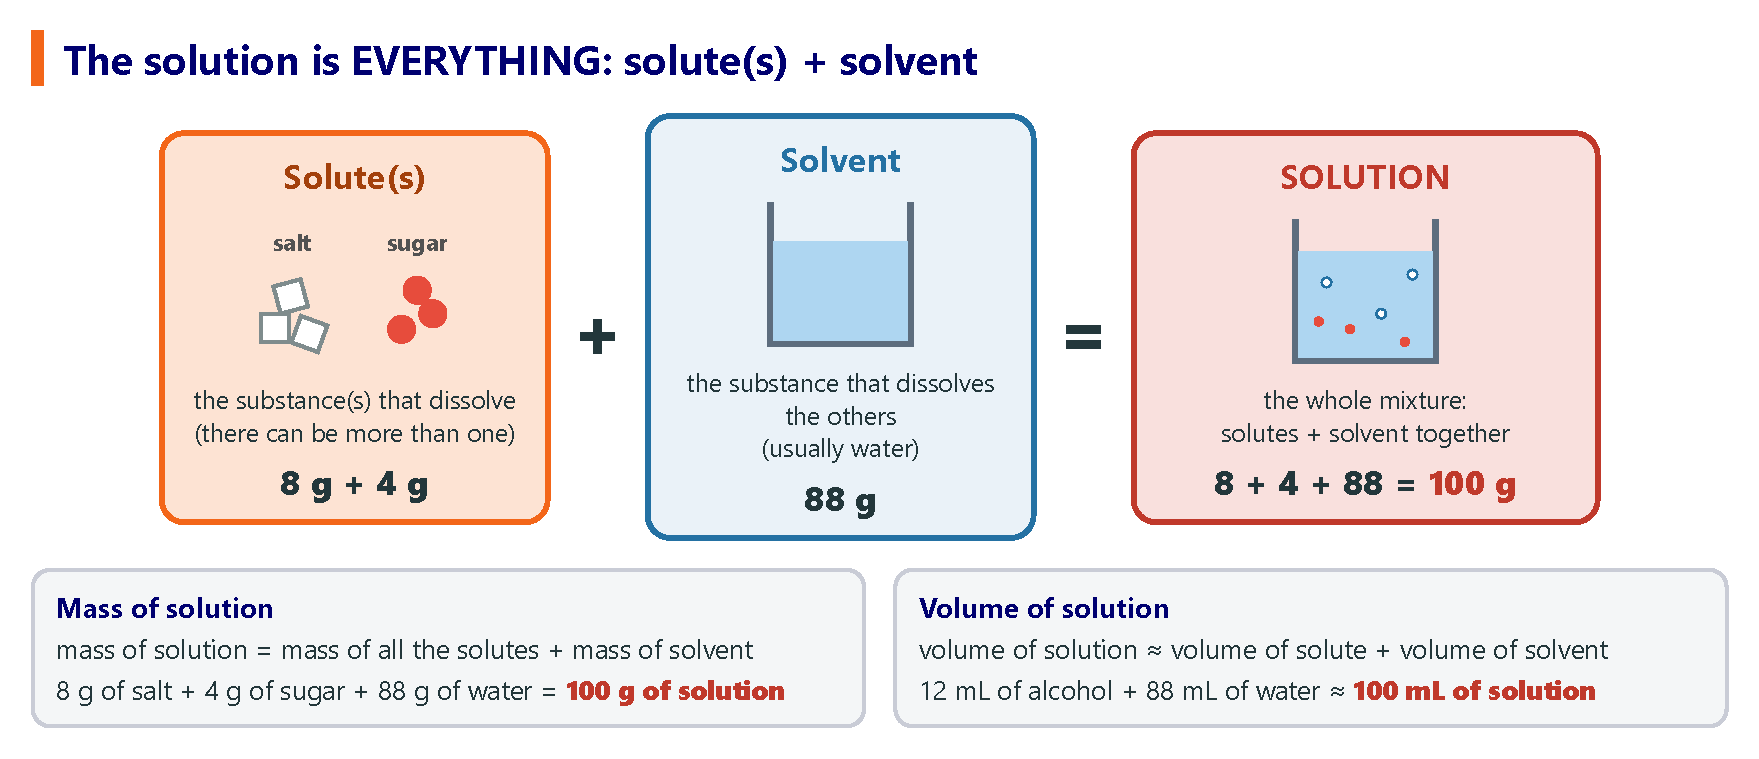
\includegraphics[width=\textwidth]{FigurasSVG/Unit_3_Diversity_of_Matter/pdf/solution_sum.pdf}
    \caption{The solution is the sum of all the solutes and the solvent.}
    \label{fig:u3_solution_sum}
\end{figure}

\begin{impt}
    \negsubro{Solution = solute(s) + solvent}
    \begin{equation*}
        \text{mass of solution} = \text{mass of solute(s)} + \text{mass of solvent}
    \end{equation*}
    \begin{equation*}
        \text{volume of solution} \approx \text{volume of solute} + \text{volume of solvent}
    \end{equation*}
    In all the formulas of concentration, the \textbf{solution} goes \textbf{below} the fraction line, \textbf{never} the solvent alone. If the exercise gives you the solute and the solvent separately, first \textbf{add them} to obtain the solution.
\end{impt}

We will use three ways of expressing the concentration of a solution:

\begin{figure}[H]
    \centering
    % [FIGURA ORIGINAL] \includegraphics[width=\textwidth]{Unit_3/concentration}
    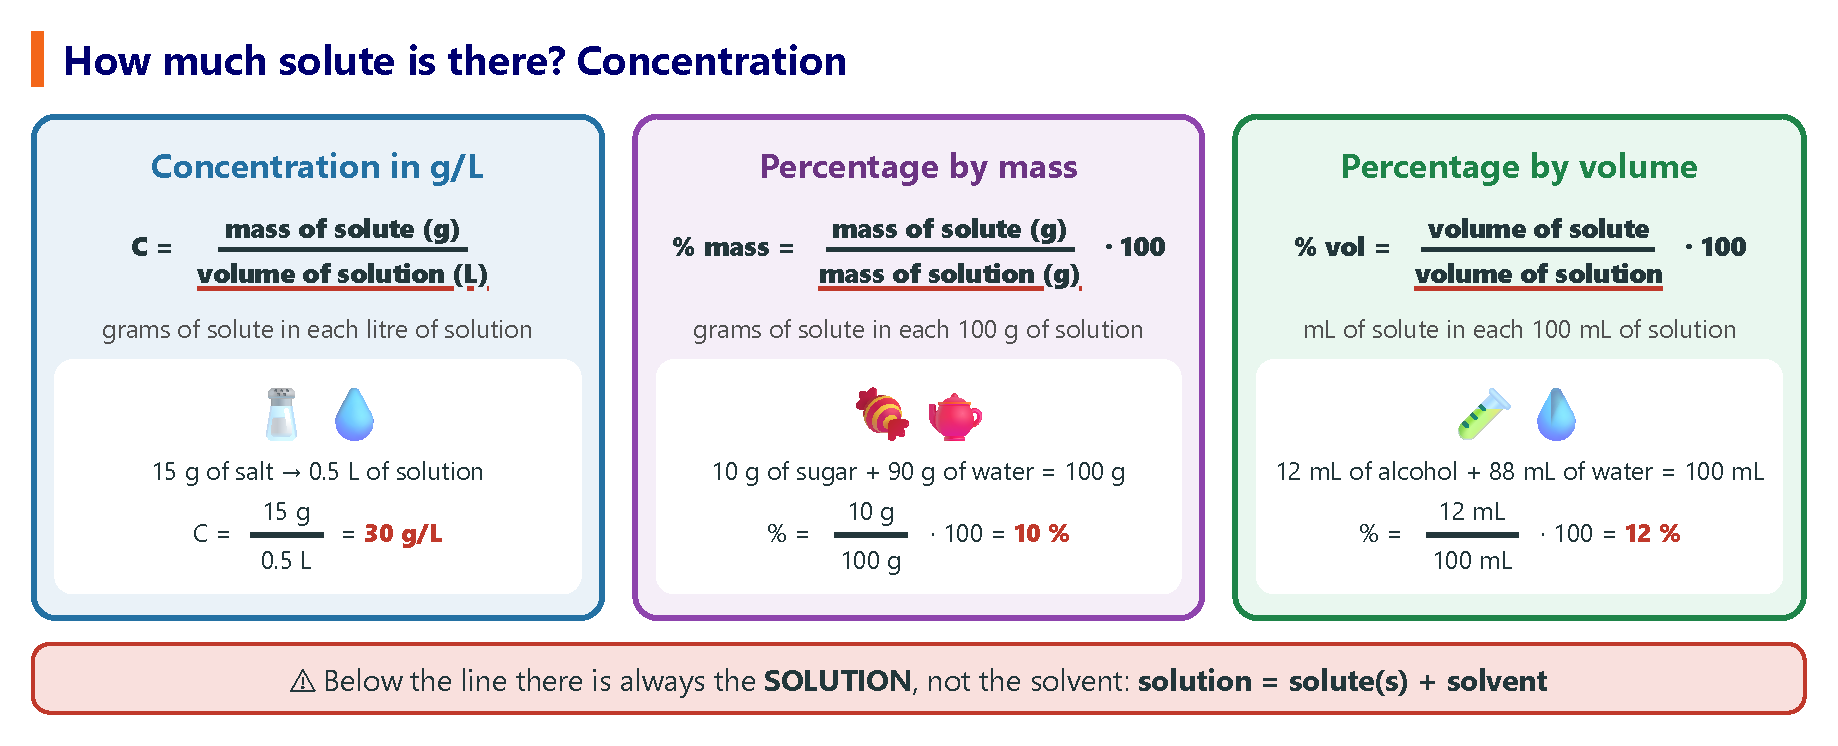
\includegraphics[width=\textwidth]{FigurasSVG/Unit_3_Diversity_of_Matter/pdf/concentration.pdf}
    \caption{Three ways of expressing concentration.}
    \label{fig:u3_concentration}
\end{figure}

\begin{equation*}
    C\,(\unit{\g\per\litre}) = \dfrac{\text{mass of solute (g)}}{\text{volume of solution (L)}}
\end{equation*}
\begin{equation*}
    \%\text{ mass} = \dfrac{\text{mass of solute (g)}}{\text{mass of solution (g)}} \cdot 100
    \qquad\qquad
    \%\text{ volume} = \dfrac{\text{volume of solute (mL)}}{\text{volume of solution (mL)}} \cdot 100
\end{equation*}

\begin{impt}
    \begin{itemize}
        \item The \textbf{concentration in g/L} tells us how many \textbf{grams} of solute there are in each \textbf{litre} of solution. The volume must be in \textbf{litres}.
        \item The \textbf{percentage by mass} tells us how many \textbf{grams} of solute there are in each \textbf{\qty{100}{\g}} of solution. Both masses must be in the \textbf{same unit}.
        \item The \textbf{percentage by volume} tells us how many \textbf{millilitres} of solute there are in each \textbf{\qty{100}{\mL}} of solution. It is used when the solute is a \textbf{liquid} (alcohol in wine, for example). Both volumes must be in the \textbf{same unit}.
    \end{itemize}
\end{impt}

\begin{example}
    \textbf{Concentration in g/L. \qty{15}{\g} of salt are dissolved in water to make \qty{500}{\mL} of solution. What is the concentration in g/L?}
    \begin{enumerate}[label=\numberballmDarkTeal]
        \item Data: mass of solute \(= \qty{15}{\g}\); volume of solution \(= \qty{500}{\mL}\). Unknown: \(C\).
        \item The volume must be in litres: \(\num{500}\,\unit{\mL} \cdot \dfrac{\qty{1}{\litre}}{\qty{e3}{\mL}} = \qty{0.5}{\litre}\).
        \item Formula: \(C = \dfrac{\text{mass of solute}}{\text{volume of solution}}\).
        \item \(C = \dfrac{\qty{15}{\g}}{\qty{0.5}{\litre}} = \textcolor{red}{\qty{30}{\g\per\litre}}\). There are \qty{30}{\g} of salt in each litre of solution.
    \end{enumerate}
\end{example}

\begin{example}
    \textbf{Percentage by mass. \qty{20}{\g} of sugar are dissolved in \qty{180}{\g} of water. What is the percentage by mass of sugar?}
    \begin{enumerate}[label=\numberballmDarkTeal]
        \item Data: mass of solute (sugar) \(= \qty{20}{\g}\); mass of \textbf{solvent} (water) \(= \qty{180}{\g}\). Unknown: \% mass.
        \item \textbf{Careful}: \qty{180}{\g} is the solvent, \textbf{not} the solution. We add them: \\
        mass of solution \(= \qty{20}{\g} + \qty{180}{\g} = \qty{200}{\g}\).
        \item Formula: \(\%\text{ mass} = \dfrac{\text{mass of solute}}{\text{mass of solution}} \cdot 100\).
        \item \(\%\text{ mass} = \dfrac{\qty{20}{\g}}{\qty{200}{\g}} \cdot 100 = \textcolor{red}{\qty{10}{\percent}}\). There are \qty{10}{\g} of sugar in each \qty{100}{\g} of solution.
    \end{enumerate}
\end{example}

\begin{example}
    \textbf{Percentage by volume. A solution is prepared by mixing \qty{30}{\mL} of alcohol with \qty{120}{\mL} of water. What is the percentage by volume of alcohol?}
    \begin{enumerate}[label=\numberballmDarkTeal]
        \item Data: volume of solute (alcohol) \(= \qty{30}{\mL}\); volume of \textbf{solvent} (water) \(= \qty{120}{\mL}\). Unknown: \% volume.
        \item Volume of solution \(= \qty{30}{\mL} + \qty{120}{\mL} = \qty{150}{\mL}\).
        \item Formula: \(\%\text{ volume} = \dfrac{\text{volume of solute}}{\text{volume of solution}} \cdot 100\).
        \item \(\%\text{ volume} = \dfrac{\qty{30}{\mL}}{\qty{150}{\mL}} \cdot 100 = \textcolor{red}{\qty{20}{\percent}}\). There are \qty{20}{\mL} of alcohol in each \qty{100}{\mL} of solution.
    \end{enumerate}
\end{example}

\begin{didyouknow}
    The labels of drinks show the percentage by volume of alcohol: ``13\,\% vol.'' on a bottle of wine means that each \qty{100}{\mL} of wine contain \qty{13}{\mL} of alcohol.
\end{didyouknow}

\begin{exercise}
    \textbf{Concentration in g/L.} Calculate:
    \begin{enumerate}[label=\letraminuscula]
        \item The concentration in g/L of a solution made by dissolving \qty{20}{\g} of sugar in water until the volume is \qty{400}{\mL}.
        \item The concentration in g/L of a solution that contains \qty{6}{\g} of salt in \qty{1.5}{\litre} of solution.
        \item The mass of salt in a \qty{500}{\mL} bottle of saline solution whose concentration is \qty{9}{\g\per\litre}.
    \end{enumerate}
    \begin{solu}
        \begin{enumerate}[label=\alph*)]
            \item \(V = \qty{400}{\mL} = \qty{0.4}{\litre}\); \(C = \dfrac{\qty{20}{\g}}{\qty{0.4}{\litre}} = \qty{50}{\g\per\litre}\).
            \item \(C = \dfrac{\qty{6}{\g}}{\qty{1.5}{\litre}} = \qty{4}{\g\per\litre}\).
            \item \(V = \qty{0.5}{\litre}\); mass of solute \(= C \cdot V = \qty{9}{\g\per\litre} \cdot \qty{0.5}{\litre} = \qty{4.5}{\g}\).
        \end{enumerate}
    \end{solu}
\end{exercise}

\begin{exercise}
    \textbf{Percentage by mass.} Calculate:
    \begin{enumerate}[label=\letraminuscula]
        \item The percentage by mass of a solution made with \qty{15}{\g} of salt and \qty{135}{\g} of water.
        \item The percentage by mass of each solute in a solution made with \qty{2}{\g} of salt, \qty{3}{\g} of sugar and \qty{95}{\g} of water.
        \item The mass of solute and the mass of water in \qty{300}{\g} of a solution at \qty{5}{\percent} by mass.
    \end{enumerate}
    \begin{solu}
        \begin{enumerate}[label=\alph*)]
            \item Mass of solution \(= 15 + 135 = \qty{150}{\g}\); \(\%\text{ mass} = \dfrac{\qty{15}{\g}}{\qty{150}{\g}} \cdot 100 = \qty{10}{\percent}\).
            \item Mass of solution \(= 2 + 3 + 95 = \qty{100}{\g}\) (all the solutes and the solvent). Salt: \(\dfrac{\qty{2}{\g}}{\qty{100}{\g}} \cdot 100 = \qty{2}{\percent}\); sugar: \(\dfrac{\qty{3}{\g}}{\qty{100}{\g}} \cdot 100 = \qty{3}{\percent}\).
            \item Mass of solute \(= \qty{300}{\g} \cdot \dfrac{5}{100} = \qty{15}{\g}\); mass of water \(= 300 - 15 = \qty{285}{\g}\).
        \end{enumerate}
    \end{solu}
\end{exercise}

\begin{exercise}
    \textbf{Percentage by volume.} Calculate:
    \begin{enumerate}[label=\letraminuscula]
        \item The percentage by volume of a solution made by mixing \qty{30}{\mL} of alcohol with \qty{220}{\mL} of water.
        \item The volume of alcohol in a \qty{750}{\mL} bottle of wine labelled ``\qty{13}{\percent} vol.''.
        \item A hand sanitiser gel has \qty{70}{\percent} alcohol by volume. How many millilitres of alcohol and of water are there in a \qty{200}{\mL} bottle?
    \end{enumerate}
    \begin{solu}
        \begin{enumerate}[label=\alph*)]
            \item Volume of solution \(= 30 + 220 = \qty{250}{\mL}\); \(\%\text{ volume} = \dfrac{\qty{30}{\mL}}{\qty{250}{\mL}} \cdot 100 = \qty{12}{\percent}\).
            \item Volume of alcohol \(= \qty{750}{\mL} \cdot \dfrac{13}{100} = \qty{97.5}{\mL}\).
            \item Alcohol: \(\qty{200}{\mL} \cdot \dfrac{70}{100} = \qty{140}{\mL}\); water: \(200 - 140 = \qty{60}{\mL}\).
        \end{enumerate}
    \end{solu}
\end{exercise}

%\begin{definition}[Solubility]
%    The \textbf{maximum} amount of solute that can dissolve in a given amount of solvent, at a given temperature. A solution with this maximum amount is \textbf{saturated}: any extra solute stays at the bottom.
%\end{definition}

%\begin{figure}[H]
%    \centering
%    % [FIGURA ORIGINAL] \includegraphics[width=\textwidth]{Unit_3/solubility_graph}
%    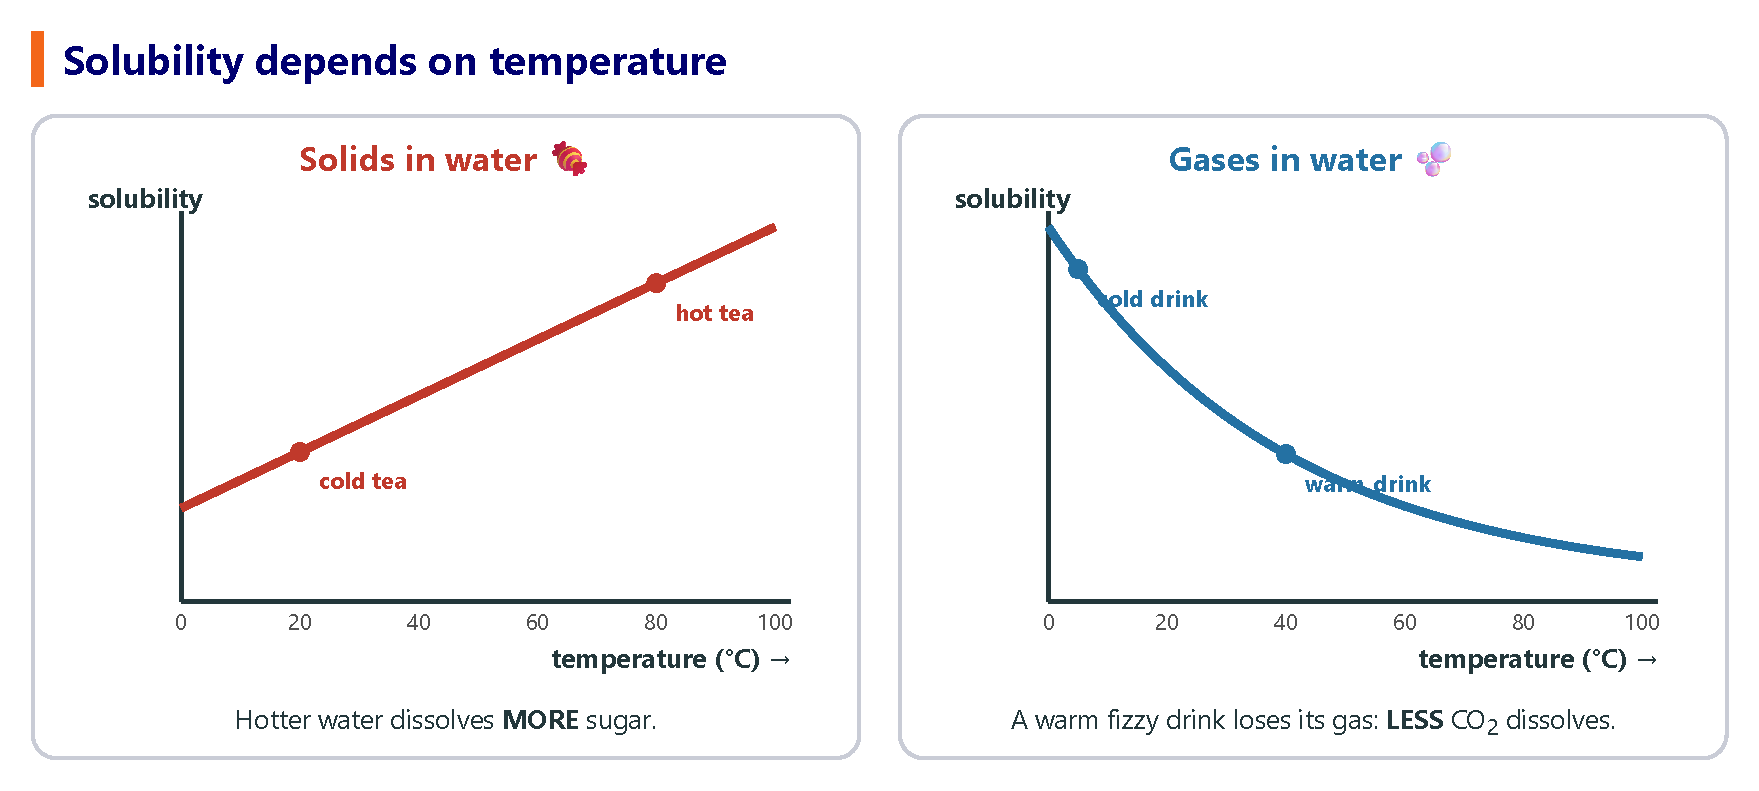
\includegraphics[width=\textwidth]{FigurasSVG/Unit_3_Diversity_of_Matter/pdf/solubility_graph.pdf}
%    \caption{Temperature increases the solubility of most solids, but decreases the solubility of gases.}
%    \label{fig:u3_solubility_graph}
%\end{figure}

%\begin{impt}
%    Solubility depends on:
%    \begin{itemize}
%        \item \textbf{The substances}: salt and sugar dissolve in water; oil and sand do not.
%        \item \textbf{Temperature}: see the graphs above.
%        \item \textbf{Stirring} does \emph{not} change the solubility, but it makes the solute dissolve \textbf{faster}.
%    \end{itemize}
%\end{impt}

\begin{exercise}
    \qty{25}{\g} of sugar are dissolved in water to make \qty{250}{\mL} of solution. Calculate the concentration of the solution in g/L.
    \begin{solu}
        \(V = \qty{250}{\mL} = \qty{0.250}{\litre}\); \quad \(C = \dfrac{\qty{25}{\g}}{\qty{0.250}{\litre}} = \qty{100}{\g\per\litre}\).
    \end{solu}
\end{exercise}

\begin{exercise}
    A solution is prepared by dissolving \qty{8}{\g} of salt in \qty{92}{\g} of water.
    \begin{enumerate}[label=\letraminuscula]
        \item Calculate the percentage by mass of the solution.
        \item If we had \qty{500}{\g} of this same solution, what mass of salt would it contain?
    \end{enumerate}
    \begin{solu}
        \begin{enumerate}[label=\alph*)]
            \item Mass of solution \(= \qty{8}{\g} + \qty{92}{\g} = \qty{100}{\g}\); \quad \(\% \text{ mass} = \dfrac{\qty{8}{\g}}{\qty{100}{\g}} \cdot 100 = \qty{8}{\percent}\).
            \item \(\qty{500}{\g} \cdot \dfrac{8}{100} = \qty{40}{\g}\) of salt.
        \end{enumerate}
    \end{solu}
\end{exercise}

\begin{exercise}
    Explain, using the idea of solubility, why sugar dissolves better in hot tea than in cold tea, and why a can of fizzy drink loses its bubbles faster when it is left open on a warm day.
    \begin{solu}
        The solubility of a solid such as sugar \textbf{increases} with temperature, so more sugar dissolves in hot tea. \\
        The solubility of a gas such as \ch{CO2} \textbf{decreases} with temperature: as the drink warms up, less gas can stay dissolved, and it escapes as bubbles.
    \end{solu}
\end{exercise}

\begin{exercise}
    A bottle contains \qty{750}{\mL} of a solution with a concentration of \qty{40}{\g\per\litre}. Calculate the mass of solute dissolved in the bottle.
    \begin{solu}
        \(\text{mass} = C \cdot V = \qty{40}{\g\per\litre} \cdot \qty{0.750}{\litre} = \qty{30}{\g}\) of solute.
    \end{solu}
\end{exercise}

\begin{exercise}
    A solution is prepared by dissolving \qty{12}{\g} of salt in enough water to make \qty{200}{\g} of solution.
    \begin{enumerate}[label=\letraminuscula]
        \item Calculate the percentage by mass of the solution.
        \item What mass of this solution would you need in order to have \qty{6}{\g} of salt?
    \end{enumerate}
    \begin{solu}
        \begin{enumerate}[label=\alph*)]
            \item \(\% \text{ mass} = \dfrac{\qty{12}{\g}}{\qty{200}{\g}} \cdot 100 = \qty{6}{\percent}\).
            \item \(\qty{6}{\g} \cdot \dfrac{100}{6} = \qty{100}{\g}\) of solution.
        \end{enumerate}
    \end{solu}
\end{exercise}

\subsection{Heterogeneous mixtures}

\begin{definition}[Heterogeneous mixture]
    A mixture whose components \textbf{can be distinguished with the naked eye}: we can see different parts in it, and two samples taken from different places may have a different composition.
\end{definition}

\begin{example}
    Some heterogeneous mixtures:
    \begin{itemize}
        \item \textbf{Granite}: we can see grains of three different minerals (white, black and pink or grey).
        \item \textbf{Sand and water}, or \textbf{muddy water}: the sand or the mud can be seen, and it settles at the bottom.
        \item \textbf{Oil and water}: two layers, with the oil on top.
        \item \textbf{A salad}, \textbf{paella} or \textbf{a pizza}: each ingredient can be recognised.
    \end{itemize}
\end{example}

Some heterogeneous mixtures are special: their components are so small that, with the naked eye, the mixture \textbf{looks} homogeneous, and we need a microscope to see its different parts. These are the \textbf{colloids}.

\subsubsection{Colloids}

\begin{definition}[Colloid]
    A heterogeneous mixture that \textbf{looks} homogeneous to the naked eye, but in which we can see particles of different composition under a microscope. Examples: milk, blood, mayonnaise, gelatine, fog.
\end{definition}

\begin{definition}[Tyndall effect]
    The scattering of light by the particles of a colloid, which makes a beam of light visible inside it. Solutions do \textbf{not} show this effect.
\end{definition}

\begin{figure}[H]
    \centering
    % [FIGURA ORIGINAL] \includegraphics[width=\textwidth]{Unit_3/tyndall}
    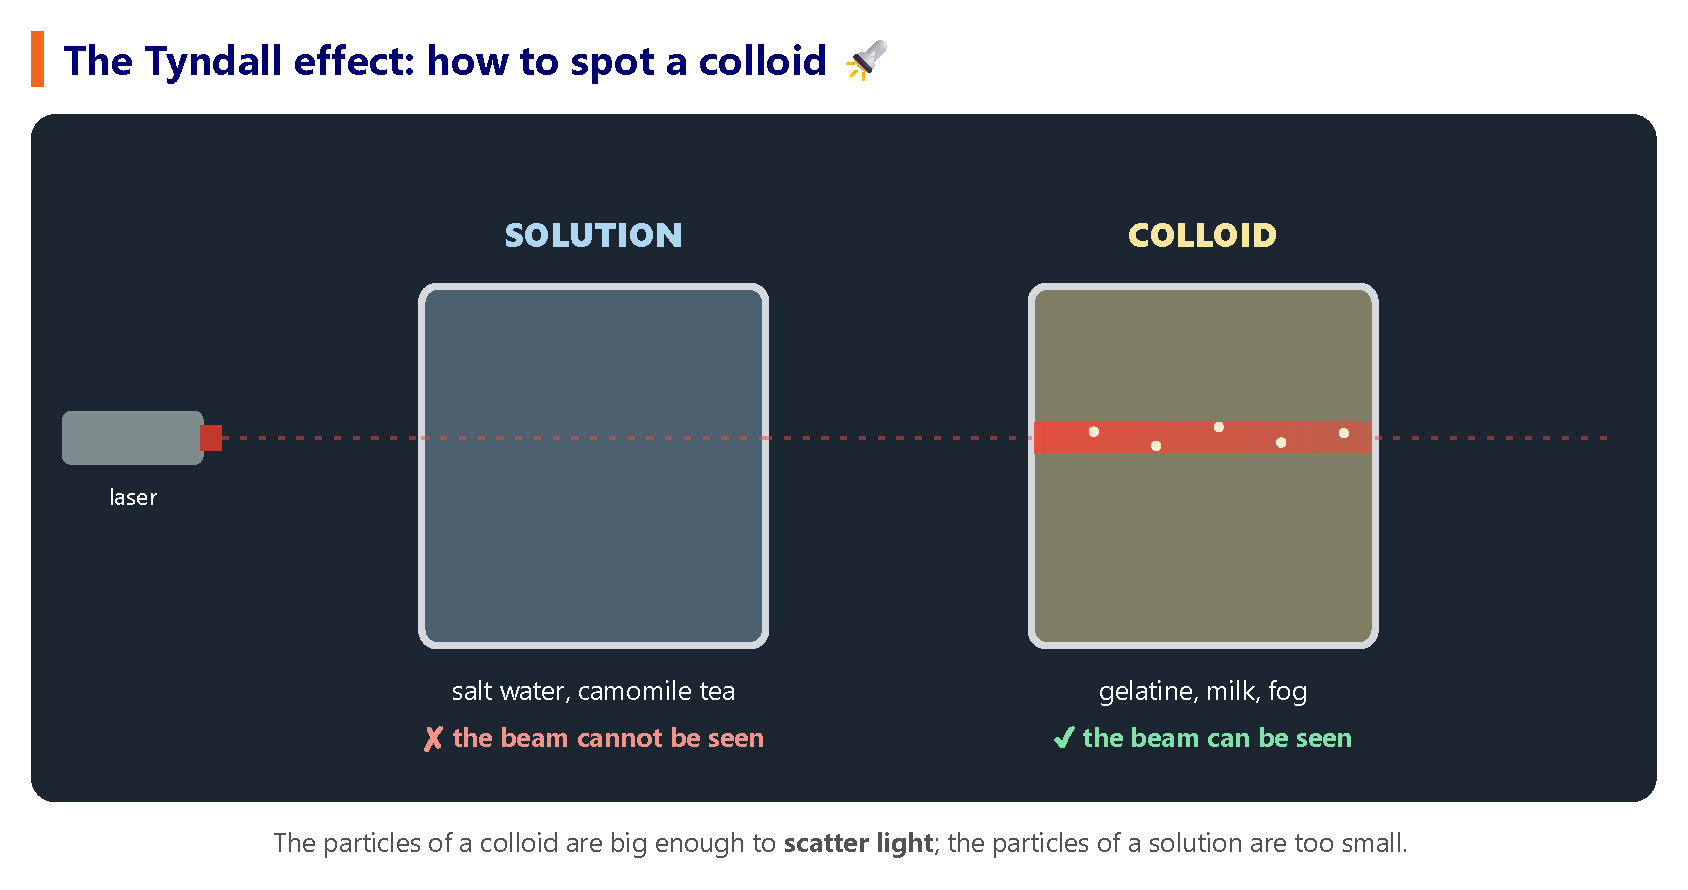
\includegraphics[width=\textwidth]{FigurasSVG/Unit_3_Diversity_of_Matter/pdf/tyndall.pdf}
    \caption{The Tyndall effect lets us tell a colloid from a solution.}
    \label{fig:u3_tyndall}
\end{figure}

\begin{didyouknow}
    When sunbeams come through the trees on a foggy morning, or through the window of a dusty room, you are seeing the Tyndall effect! Fog and dusty air are colloids, and their particles scatter the sunlight.
\end{didyouknow}

\begin{exercise}
    Explain why a solution of copper sulphate in water does not show the Tyndall effect, while a mixture of gelatine in water does.
    \begin{solu}
        In the copper sulphate solution the dissolved particles are extremely small, too small to scatter light, so the beam is not visible. In gelatine, the particles are larger (colloid size) and scatter the light, so the beam can be seen: this is the \textbf{Tyndall effect}.
    \end{solu}
\end{exercise}

\begin{exercise}
    Classify each mixture as a \textbf{solution} or a \textbf{colloid}, giving a reason based on particle size: mayonnaise, sea water, whipped cream, vinegar.
    \begin{solu}
        Mayonnaise: \textbf{colloid} (oil droplets dispersed in water). \\
        Sea water: \textbf{solution} (dissolved salts, very small particles). \\
        Whipped cream: \textbf{colloid} (tiny air bubbles and fat droplets). \\
        Vinegar: \textbf{solution} (acetic acid dissolved in water).
    \end{solu}
\end{exercise}

\subsubsection{Emulsions}

\begin{definition}[Emulsion]
    A colloid made of two liquids that do not mix (such as oil and water), kept together by a third substance called an \textbf{emulsifier}.
\end{definition}

\begin{figure}[H]
    \centering
    % [FIGURA ORIGINAL] \includegraphics[width=\textwidth]{Unit_3/emulsion}
    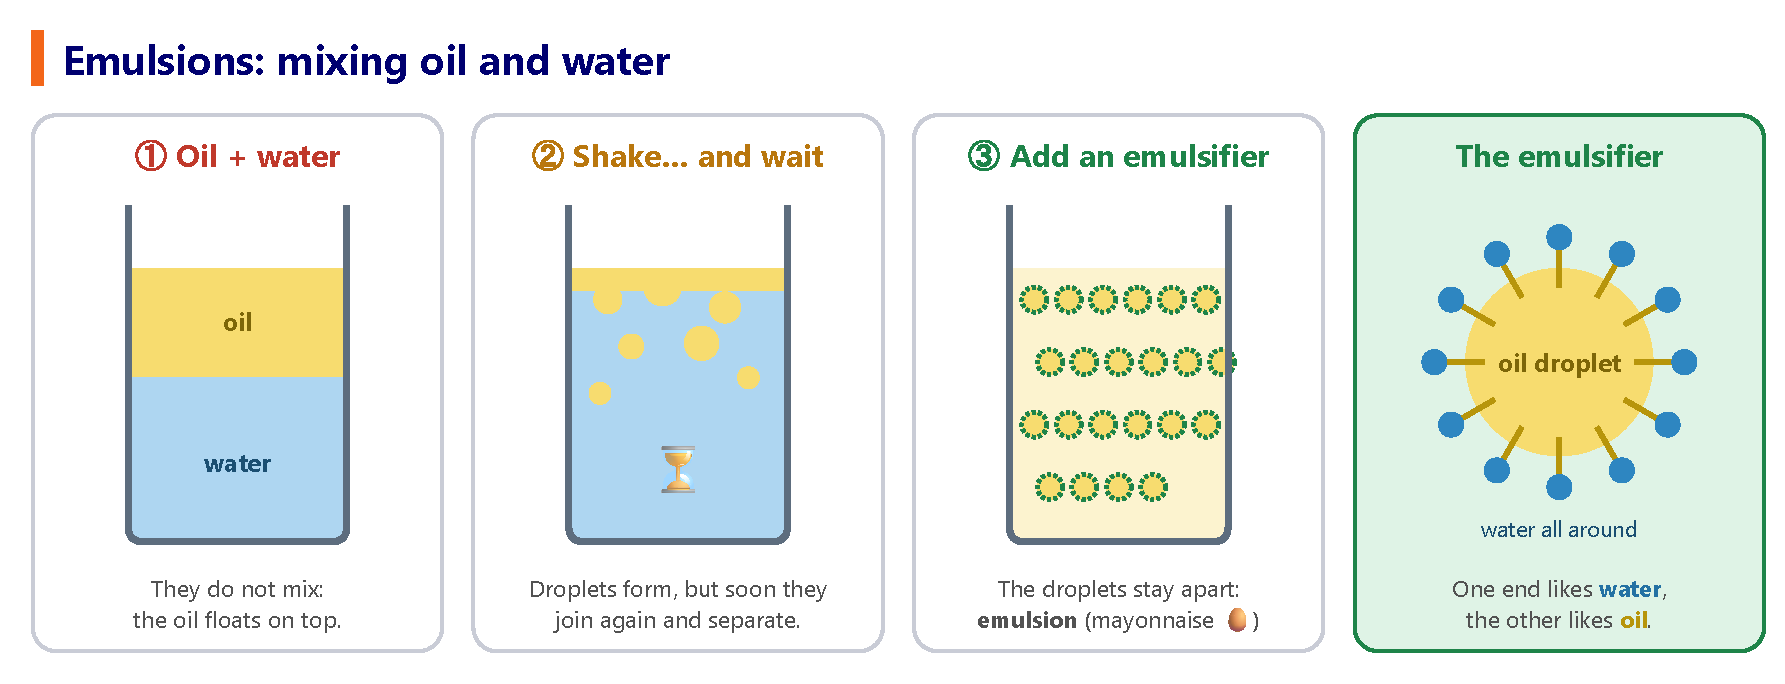
\includegraphics[width=\textwidth]{FigurasSVG/Unit_3_Diversity_of_Matter/pdf/emulsion.pdf}
    \caption{An emulsifier keeps the oil droplets apart inside the water.}
    \label{fig:u3_emulsion}
\end{figure}

\begin{example}
    In mayonnaise the emulsifier is \textbf{lecithin}, from egg yolk; in milk it is \textbf{casein}, a milk protein. Soap also works as an emulsifier: that is why it removes grease from your hands.
\end{example}

\begin{exercise}
    Explain what happens if you shake a mixture of oil and water \textbf{without} adding any emulsifier, and why.
    \begin{solu}
        Shaking breaks the oil into small droplets, but without an emulsifier nothing keeps them apart. The droplets join together again and the mixture separates into two layers, with the less dense oil on top.
    \end{solu}
\end{exercise}

\begin{exercise}
    Identify the emulsifier in each emulsion: a) mayonnaise; b) milk; c) many cosmetic creams.
    \begin{solu}
        \begin{enumerate}[label=\alph*)]
            \item Lecithin, from egg yolk.
            \item Casein, a milk protein.
            \item Emulsifying waxes or soap-like molecules, with one end that mixes with water and the other with oil.
        \end{enumerate}
    \end{solu}
\end{exercise}

\subsection{Particle size and types of mixtures}

\begin{figure}[H]
    \centering
    % [FIGURA ORIGINAL] \includegraphics[width=\textwidth]{Unit_3/particle_size}
    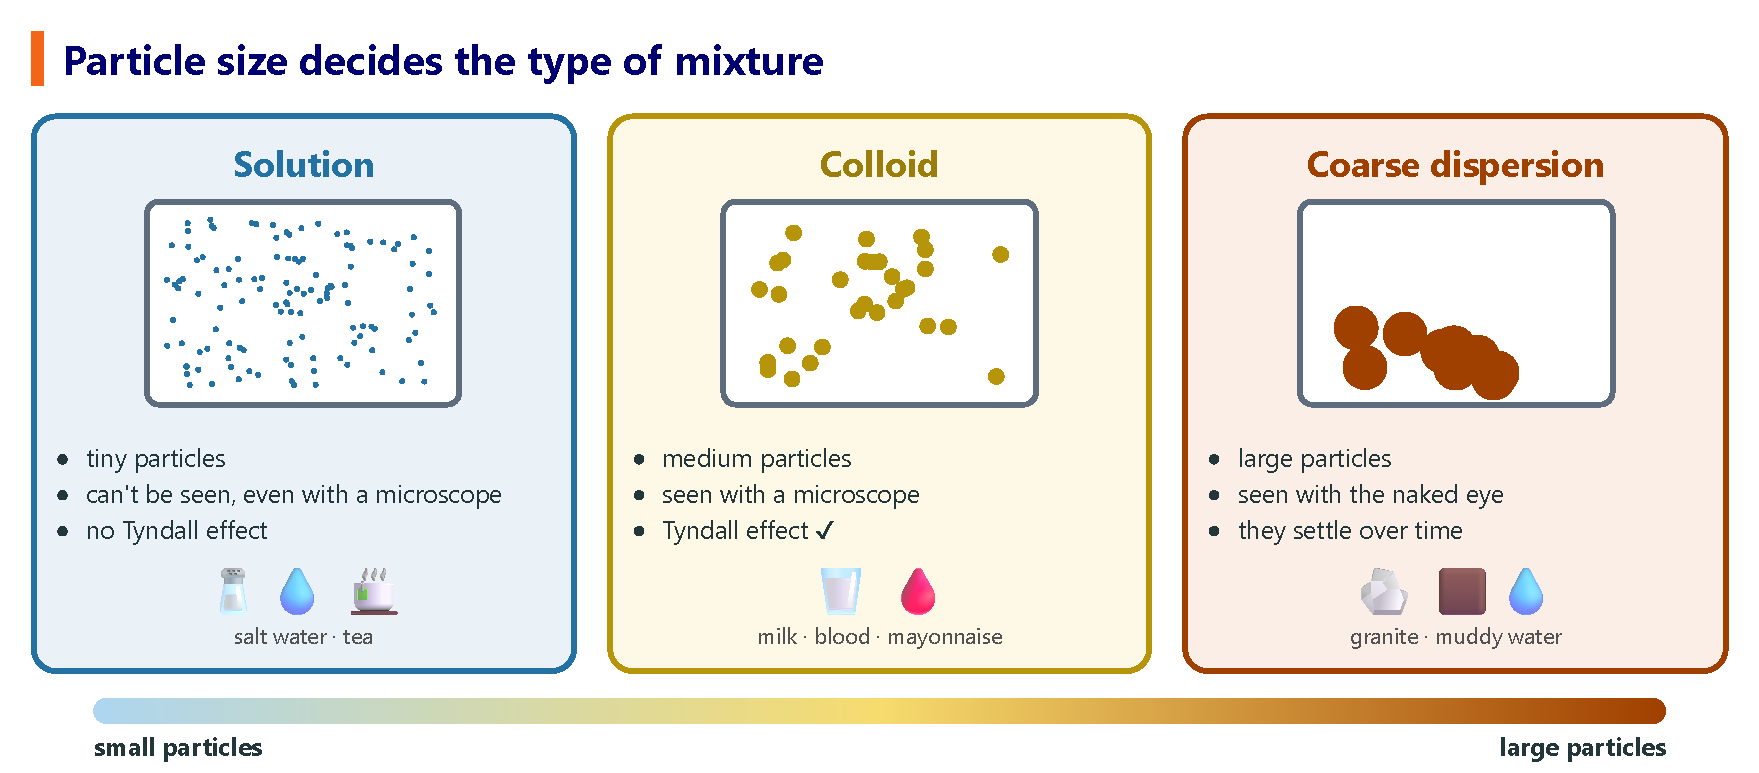
\includegraphics[width=\textwidth]{FigurasSVG/Unit_3_Diversity_of_Matter/pdf/particle_size.pdf}
    \caption{The bigger the dispersed particles, the more heterogeneous the mixture.}
    \label{fig:u3_particle_size}
\end{figure}

\begin{exercise}
    Classify these mixtures as homogeneous or heterogeneous, and say if they are colloids: meringue, physiological saline solution, coins (metal alloy), marble, milk, fizzy drinks.
    \begin{solu}
        Meringue: \textbf{heterogeneous}, colloid (air trapped in egg white). \\
        Physiological saline solution: \textbf{homogeneous} (a solution). \\
        Coins: \textbf{homogeneous} (an alloy, a solid solution). \\
        Marble: \textbf{heterogeneous} (we can see veins and grains). \\
        Milk: \textbf{heterogeneous}, colloid, although it looks homogeneous. \\
        Fizzy drinks: \textbf{homogeneous} (a solution of \ch{CO2} in water).
    \end{solu}
\end{exercise}

\begin{exercise}
    Order these three systems from \textbf{smallest} to \textbf{largest} dispersed-particle size, and name the type of mixture each one is: sugar solution, muddy river water, milk.
    \begin{solu}
        \textbf{Sugar solution} (solution) \(<\) \textbf{milk} (colloid) \(<\) \textbf{muddy river water} (coarse dispersion).
    \end{solu}
\end{exercise}

%----------------------------------------------------------------------------------------

\section{What makes up matter}

\begin{definition}[Atom]
    The tiny particle that makes up all matter. Atoms are made of even smaller particles: \textbf{protons}, \textbf{neutrons} and \textbf{electrons}.
\end{definition}

Scientists could not see atoms, so they imagined \textbf{models} to explain the results of their experiments. Each new experiment improved the model:

\begin{figure}[H]
    \centering
    % [FIGURA ORIGINAL] \includegraphics[width=\textwidth]{Unit_3/atomic_models}
    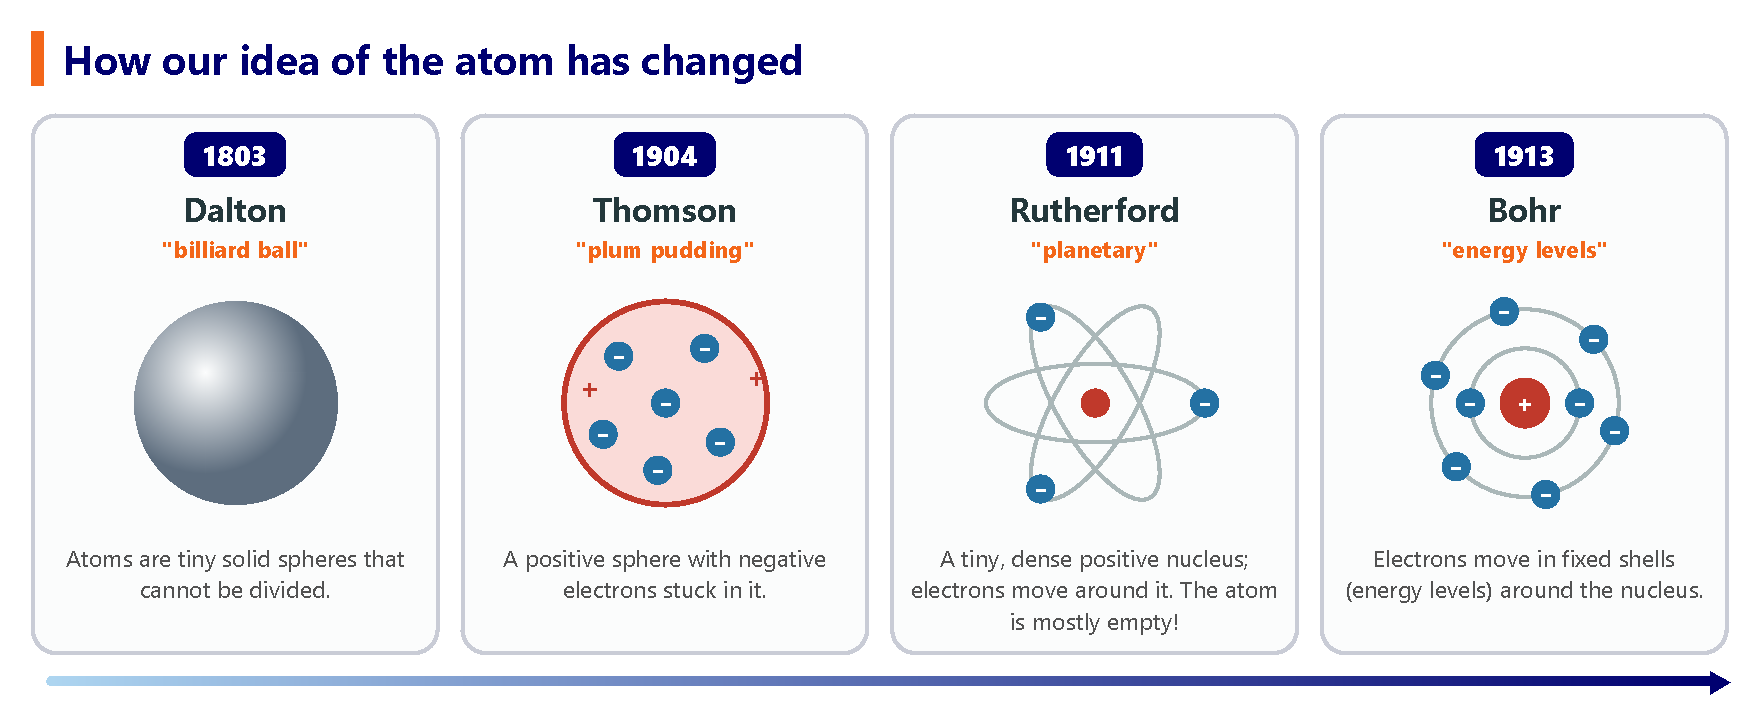
\includegraphics[width=\textwidth]{FigurasSVG/Unit_3_Diversity_of_Matter/pdf/atomic_models.pdf}
    \caption{The main atomic models.}
    \label{fig:u3_atomic_models}
\end{figure}

\begin{didyouknow}
    The atom is almost completely empty! If the nucleus were the size of a football in the centre of a stadium, the electrons would be like tiny grains of sand moving around the last rows of seats. Rutherford discovered this in 1911, when he fired particles at a very thin sheet of gold and almost all of them went straight through.
\end{didyouknow}

\subsection{The structure of the atom}

\begin{figure}[H]
    \centering
    % [FIGURA ORIGINAL] \includegraphics[width=\textwidth]{Unit_3/atom_structure}
    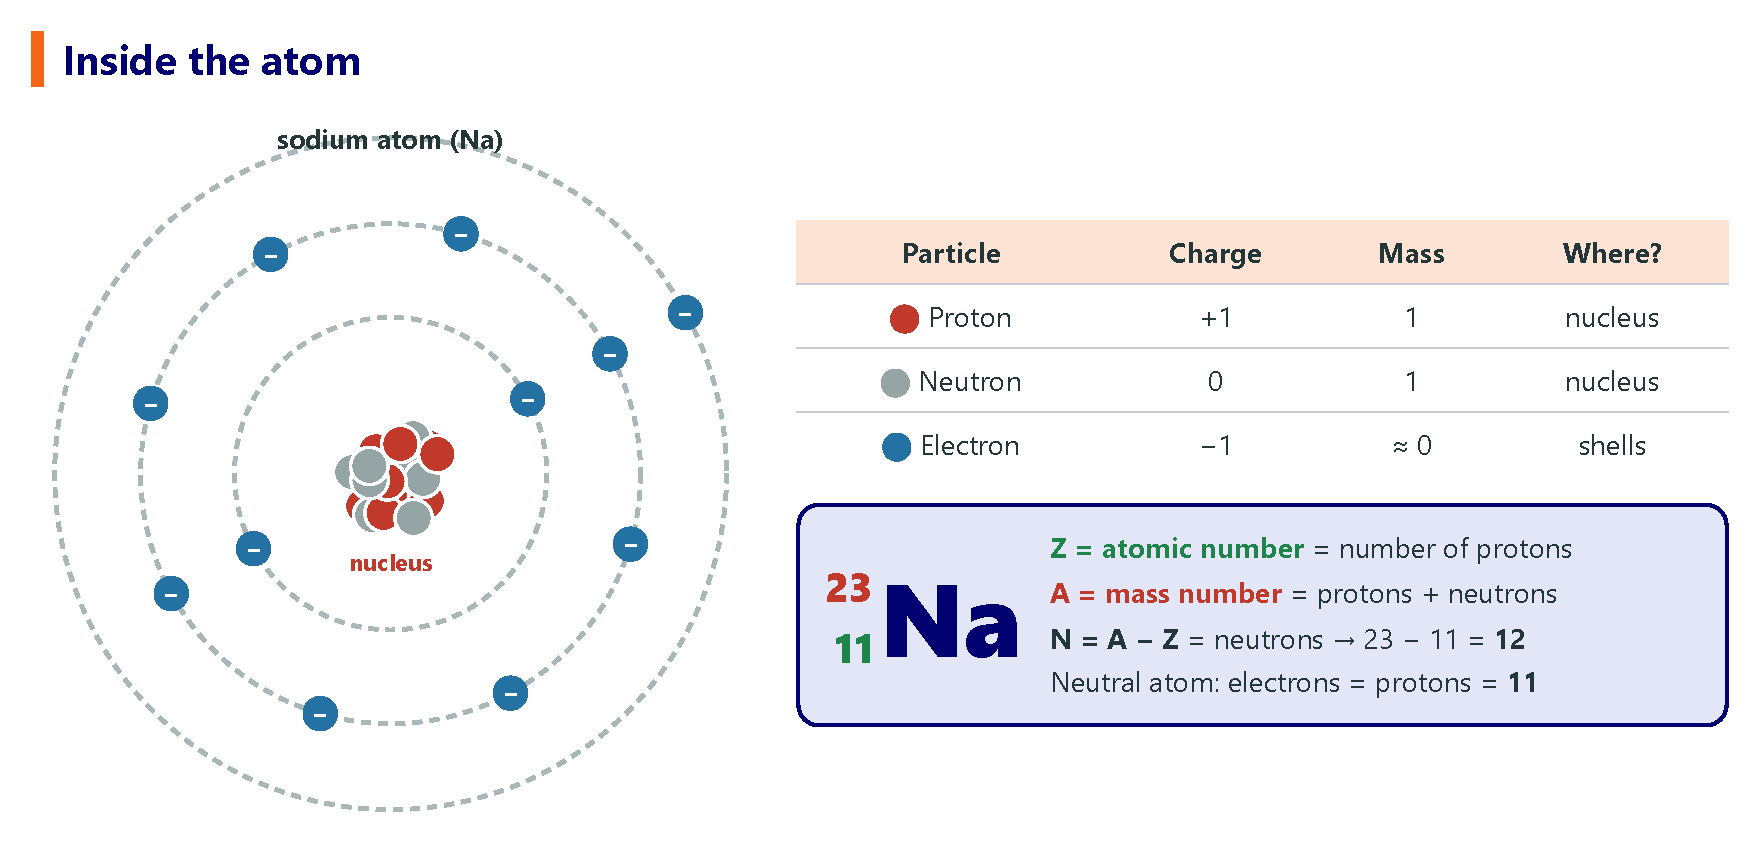
\includegraphics[width=\textwidth]{FigurasSVG/Unit_3_Diversity_of_Matter/pdf/atom_structure.pdf}
    \caption{The particles of the atom and how we represent an atom.}
    \label{fig:u3_atom_structure}
\end{figure}

\begin{impt}
    Almost all the \textbf{mass} of the atom is in the \textbf{nucleus}; almost all its \textbf{volume} is the space where the electrons move. In a \textbf{neutral} atom, number of electrons \(=\) number of protons.
\end{impt}

\begin{definition}[Atomic number \(Z\) and mass number \(A\)]
    \(Z\) is the number of \textbf{protons}: it tells us which element the atom is. \(A\) is the number of protons \textbf{plus} neutrons. So the number of neutrons is
    \begin{equation*}
        N = A - Z
    \end{equation*}
\end{definition}

\begin{example}
    Sodium, \ch{^{23}_{11}Na}: \(Z = 11\) and \(A = 23\). It has 11 protons, 11 electrons (it is neutral) and \(N = 23 - 11 = 12\) neutrons.
\end{example}

\begin{definition}[Isotopes]
    Atoms of the \textbf{same} element (same \(Z\)) with a \textbf{different} number of neutrons (different \(A\)).
\end{definition}

\begin{figure}[H]
    \centering
    % [FIGURA ORIGINAL] \includegraphics[width=0.9\textwidth]{Unit_3/isotopes}
    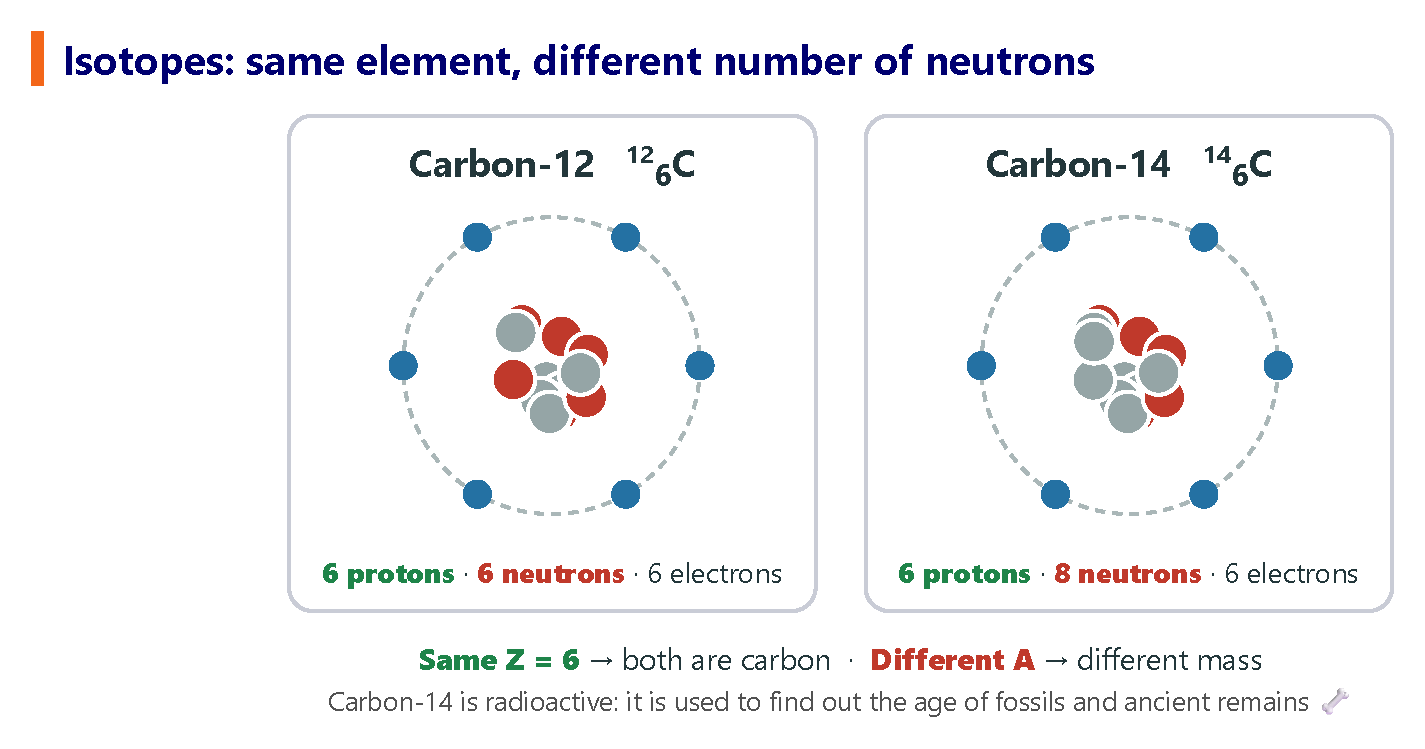
\includegraphics[width=0.9\textwidth]{FigurasSVG/Unit_3_Diversity_of_Matter/pdf/isotopes.pdf}
    \caption{Two isotopes of carbon.}
    \label{fig:u3_isotopes}
\end{figure}

\begin{exercise}
    An atom has 17 protons, 17 electrons and 18 neutrons.
    \begin{enumerate}[label=\letraminuscula]
        \item Give its atomic number \(Z\) and its mass number \(A\).
        \item Which chemical element is it? (Hint: atomic number 17 is chlorine.)
    \end{enumerate}
    \begin{solu}
        \begin{enumerate}[label=\alph*)]
            \item \(Z = 17\); \(A = 17 + 18 = 35\).
            \item \textbf{Chlorine}, \ch{Cl}.
        \end{enumerate}
    \end{solu}
\end{exercise}

\begin{exercise}
    Two isotopes of an element have mass numbers 35 and 37, and both have \(Z = 17\). Explain what they have in common and what makes them different.
    \begin{solu}
        Both have 17 protons and 17 electrons (same element). They have a different number of neutrons: \(N = 35 - 17 = 18\) and \(N = 37 - 17 = 20\).
    \end{solu}
\end{exercise}

\begin{exercise}
    Complete the table for these neutral atoms:
    \begin{center}
        \renewcommand{\arraystretch}{1.3}
        \begin{tabular}{cccccc}
            \toprule
            \textbf{Element} & \(Z\) & \(A\) & \textbf{Protons} & \textbf{Neutrons} & \textbf{Electrons} \\
            \midrule
            Oxygen & 8 & 16 & & & \\
            Magnesium & 12 & 24 & & & \\
            Potassium & 19 & 39 & & & \\
            \bottomrule
        \end{tabular}
    \end{center}
    \begin{solu}
        Oxygen: 8 protons, \(16 - 8 = 8\) neutrons, 8 electrons. \\
        Magnesium: 12 protons, \(24 - 12 = 12\) neutrons, 12 electrons. \\
        Potassium: 19 protons, \(39 - 19 = 20\) neutrons, 19 electrons.
    \end{solu}
\end{exercise}

\begin{exercise}
    Potassium-40 (\(Z = 19\), \(A = 40\)) and calcium-40 (\(Z = 20\), \(A = 40\)) have the same mass number. Explain why they are \textbf{not} isotopes, and calculate the number of neutrons in each atom.
    \begin{solu}
        Isotopes must have the \textbf{same} \(Z\). Here \(Z\) is different (19 and 20), so they are different elements. \\
        Neutrons: potassium-40, \(N = 40 - 19 = 21\); calcium-40, \(N = 40 - 20 = 20\).
    \end{solu}
\end{exercise}

\subsection{Elements, molecules and crystals}

\begin{definition}[Chemical element]
    All the atoms with the same number of protons (\(Z\)). There are 118 known elements, arranged in the periodic table.
\end{definition}

\begin{figure}[H]
    \centering
    % [FIGURA ORIGINAL] \includegraphics[width=\textwidth]{Unit_3/particle_arrangements}
    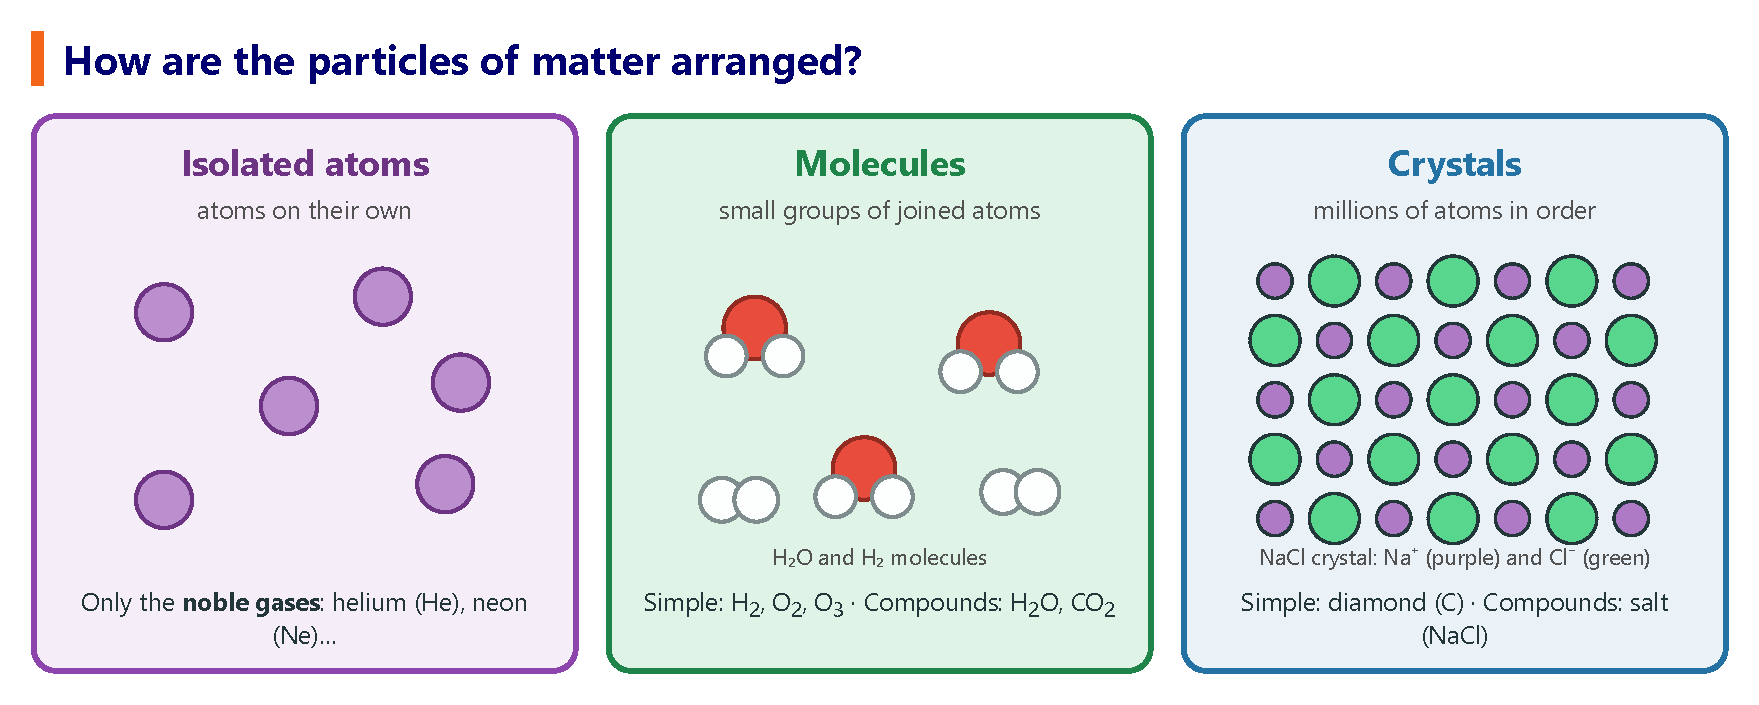
\includegraphics[width=\textwidth]{FigurasSVG/Unit_3_Diversity_of_Matter/pdf/particle_arrangements.pdf}
    \caption{The three ways in which the particles of a substance can be arranged.}
    \label{fig:u3_particle_arrangements}
\end{figure}

\begin{impt}
    \negsubro{Mixture vs.\ compound}: hydrogen gas (\ch{H2}) and oxygen gas (\ch{O2}) can be mixed in \textbf{any} proportion: that is a mixture. In water (\ch{H2O}) there are \textbf{always} 2 hydrogen atoms for each oxygen atom: that is a compound, and its properties are completely different from those of the two gases.
\end{impt}

\begin{exercise}
    Look at the three boxes in the figure below.
    \begin{figure}[H]
        \centering
        % [FIGURA ORIGINAL] \includegraphics[width=0.95\textwidth]{Unit_3/substances_particles}
        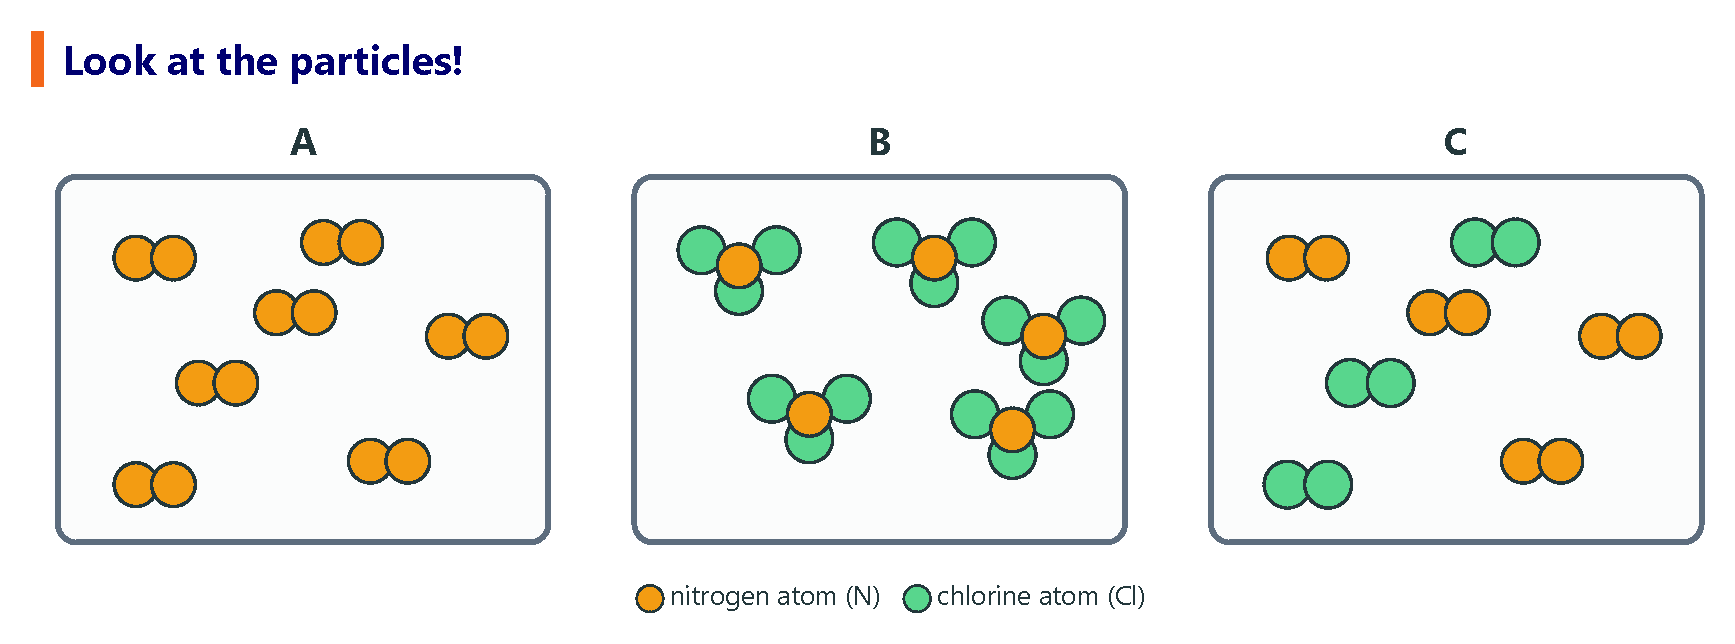
\includegraphics[width=0.95\textwidth]{FigurasSVG/Unit_3_Diversity_of_Matter/pdf/substances_particles.pdf}
    \end{figure}
    Which box shows: a) a simple substance; b) a compound; c) a mixture? Explain how you know.
    \begin{solu}
        \begin{enumerate}[label=\alph*)]
            \item \textbf{A}: all the molecules are identical (\ch{N2}) and made of only one type of atom.
            \item \textbf{B}: all the molecules are identical (\ch{NCl3}), but each one has two types of atom.
            \item \textbf{C}: there are two different types of molecules (\ch{N2} and \ch{Cl2}).
        \end{enumerate}
    \end{solu}
\end{exercise}

\begin{exercise}
    Classify as a simple substance or a compound, and as made of molecules or a crystal: diamond (\ch{C}), sodium chloride (\ch{NaCl}), hydrogen gas (\ch{H2}), water (\ch{H2O}).
    \begin{solu}
        Diamond: simple substance, crystal. \\
        Sodium chloride: compound, crystal. \\
        Hydrogen gas: simple substance, molecules. \\
        Water: compound, molecules.
    \end{solu}
\end{exercise}

\begin{exercise}
    State whether each of these is made up of \textbf{isolated atoms}, \textbf{molecules} or a \textbf{crystal}: neon gas (\ch{Ne}); carbon dioxide gas (\ch{CO2}); a diamond (\ch{C}); common salt (\ch{NaCl}).
    \begin{solu}
        Neon: \textbf{isolated atoms} (noble gas). Carbon dioxide: \textbf{molecules}. Diamond: \textbf{crystal}. Common salt: \textbf{crystal}.
    \end{solu}
\end{exercise}

%----------------------------------------------------------------------------------------

\section{The periodic table of elements}

\begin{definition}[Periodic table]
    A table with the 118 known elements, in order of increasing \textbf{atomic number} \(Z\). The rows are called \negsubro{periods} (7) and the columns \negsubro{groups} (18).
\end{definition}

\begin{figure}[H]
    \centering
    % [FIGURA ORIGINAL] \includegraphics[width=\textwidth]{Unit_3/periodic_table}
    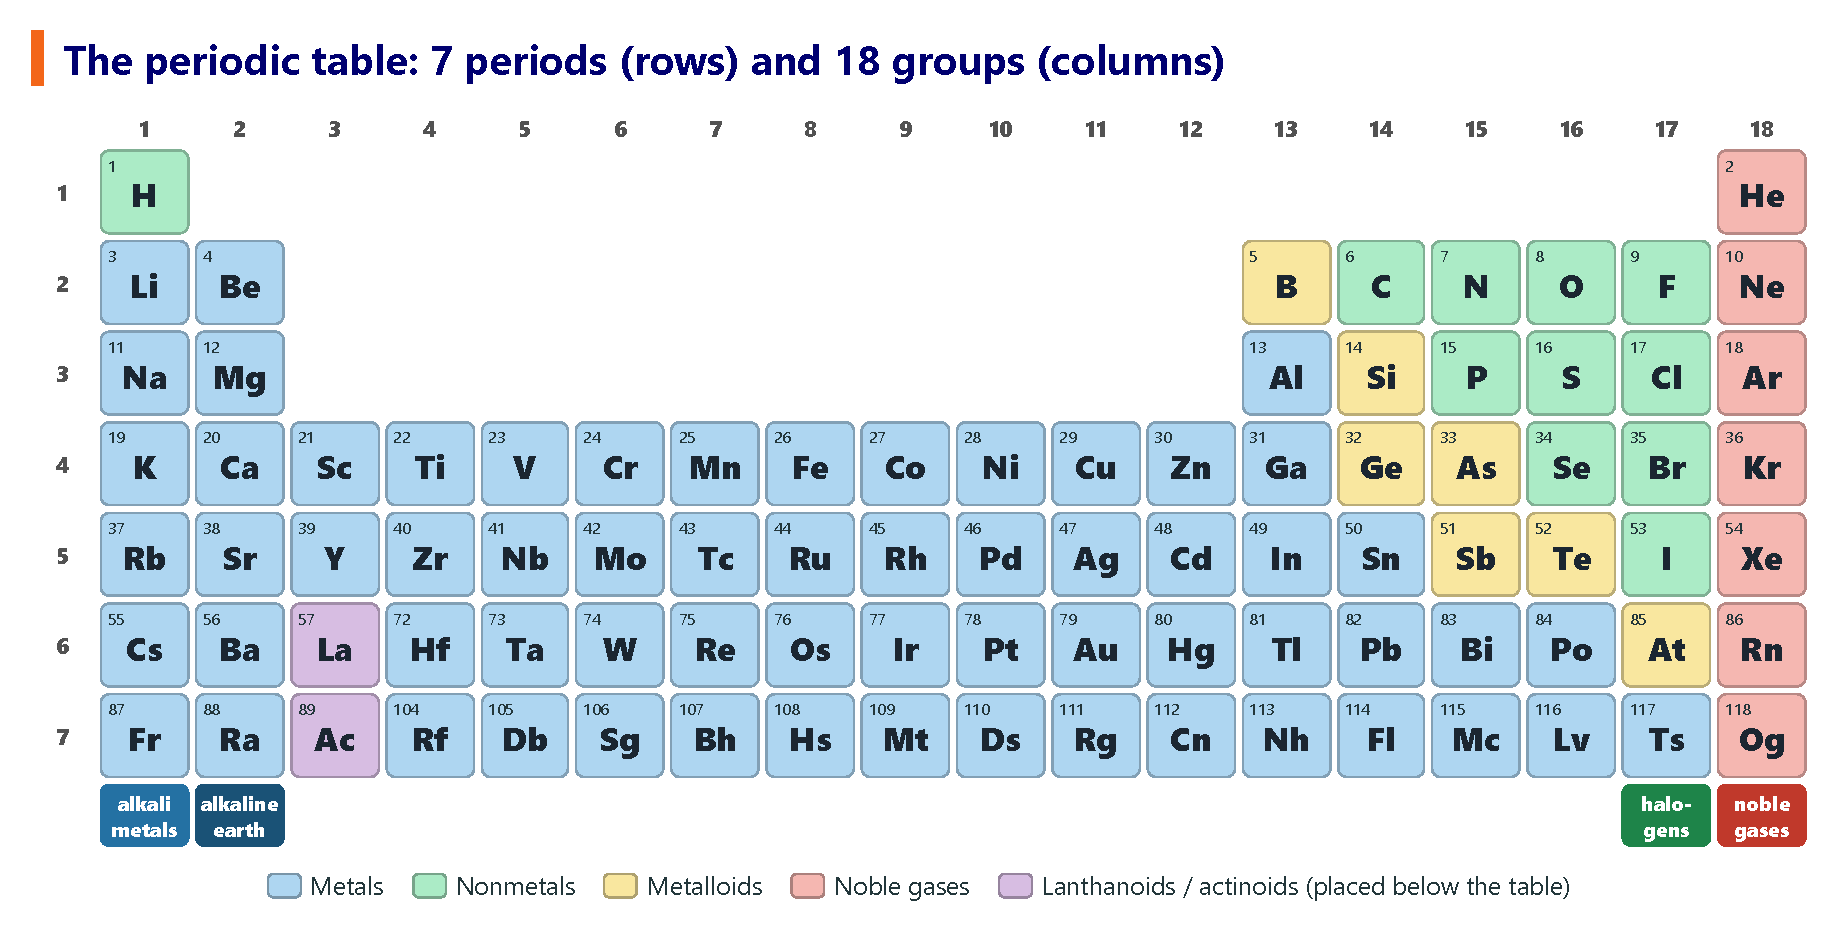
\includegraphics[width=\textwidth]{FigurasSVG/Unit_3_Diversity_of_Matter/pdf/periodic_table.pdf}
    \caption{The periodic table: metals, nonmetals, metalloids and noble gases.}
    \label{fig:u3_periodic_table}
\end{figure}

\begin{impt}
    \begin{itemize}
        \item Each element has a \textbf{symbol}: the first letter is always a capital, the second (if there is one) is lower case: \ch{H}, \ch{Ca}, \ch{Cl}.
        \item Elements in the same \textbf{group} have \textbf{similar properties}.
        \item The \textbf{period} number tells us how many electron shells the atoms have.
    \end{itemize}
\end{impt}

\begin{table}[H]
    \centering
    \small
    \renewcommand{\arraystretch}{1.35}
    \begin{tabular}{lp{9.5cm}}
        \toprule
        \textbf{Type} & \textbf{Properties} \\
        \midrule
        Metals & Most elements. Shiny, solid at room temperature (except mercury), good conductors of heat and electricity. \\
        Nonmetals & Poor conductors; many are gases (\ch{O2}, \ch{N2}) or brittle solids (\ch{S}, \ch{C}). \\
        Metalloids & Intermediate properties (silicon, used in computer chips). \\
        Noble gases & Group 18. Very stable: they almost never react. \\
        \bottomrule
    \end{tabular}
    \caption{Types of elements in the periodic table.}
    \label{tab:u3_element_types}
\end{table}

\begin{didyouknow}
    Dmitri Mendeleev organised the first periodic table in 1869. He left empty gaps for elements that nobody had discovered yet, and even predicted their properties. Years later, gallium and germanium were discovered\ldots{} and they fitted perfectly!
\end{didyouknow}

\begin{exercise}
    Use the periodic table to give the name and symbol of: the element with atomic number 6; the element with atomic number 17; the noble gas in period 2.
    \begin{solu}
        \(Z = 6\): \textbf{carbon}, \ch{C}. \quad \(Z = 17\): \textbf{chlorine}, \ch{Cl}. \quad Noble gas in period 2: \textbf{neon}, \ch{Ne}.
    \end{solu}
\end{exercise}

\begin{exercise}
    Say whether each element is a metal, a nonmetal, a metalloid or a noble gas: sodium (\ch{Na}), oxygen (\ch{O}), silicon (\ch{Si}), argon (\ch{Ar}), iron (\ch{Fe}).
    \begin{solu}
        Sodium: metal. Oxygen: nonmetal. Silicon: metalloid. Argon: noble gas. Iron: metal.
    \end{solu}
\end{exercise}

\begin{exercise}
    Elements X, Y and Z are in the same \textbf{period}, but in different groups. What does this tell you about the number of electron shells in their atoms? Are they the same element?
    \begin{solu}
        They have the \textbf{same number of electron shells} (equal to the period number). They are \textbf{not} the same element: being in different groups, they have different atomic numbers.
    \end{solu}
\end{exercise}

\subsection{Some important groups}

\begin{table}[H]
    \centering
    \small
    \renewcommand{\arraystretch}{1.35}
    \begin{tabular}{lcp{7.5cm}}
        \toprule
        \textbf{Name} & \textbf{Group} & \textbf{Examples and properties} \\
        \midrule
        Alkali metals & 1 & \ch{Li}, \ch{Na}, \ch{K}: very reactive metals (they react violently with water). \\
        Alkaline earth metals & 2 & \ch{Mg}, \ch{Ca}: reactive metals. \\
        Halogens & 17 & \ch{F}, \ch{Cl}, \ch{Br}, \ch{I}: very reactive nonmetals. \\
        Noble gases & 18 & \ch{He}, \ch{Ne}, \ch{Ar}: very unreactive gases. \\
        \bottomrule
    \end{tabular}
    \caption{Some important groups of the periodic table.}
    \label{tab:u3_groups}
\end{table}

\begin{exercise}
    Name the group to which each element belongs, and say whether it is likely to be very reactive or very unreactive: potassium (\ch{K}), neon (\ch{Ne}), chlorine (\ch{Cl}).
    \begin{solu}
        Potassium: \textbf{alkali metal} (group 1), very reactive. \\
        Neon: \textbf{noble gas} (group 18), very unreactive. \\
        Chlorine: \textbf{halogen} (group 17), very reactive.
    \end{solu}
\end{exercise}

\begin{exercise}
    Sodium (\ch{Na}) and potassium (\ch{K}) both belong to group 1. Predict whether they react with water in a similar way, and explain why.
    \begin{solu}
        Yes. Elements in the same group have similar chemical properties. Both are \textbf{alkali metals}, so both react vigorously with water, producing hydrogen gas and a metal hydroxide.
    \end{solu}
\end{exercise}

\begin{exercise}
    Classify each element as an alkali metal, alkaline earth metal, halogen or noble gas: lithium (\ch{Li}), fluorine (\ch{F}), calcium (\ch{Ca}), krypton (\ch{Kr}), bromine (\ch{Br}).
    \begin{solu}
        Lithium: alkali metal. Fluorine: halogen. Calcium: alkaline earth metal. Krypton: noble gas. Bromine: halogen.
    \end{solu}
\end{exercise}

%----------------------------------------------------------------------------------------
%
%\section{How chemical compounds are named}
%
%\subsection{Binary compounds}
%
%\begin{definition}[Binary compound]
%    A compound made of atoms of \textbf{two} different elements (for example, oxides: oxygen + another element).
%\end{definition}
%
%\begin{figure}[H]
%    \centering
%    \includegraphics[width=\textwidth]{Unit_3/naming}
%    \caption{Naming compounds with prefixes.}
%    \label{fig:u3_naming}
%\end{figure}
%
%\begin{impt}
%    \negsubro{Rules}:
%    \begin{enumerate}[label=\numberballmDarkTeal]
%        \item In the \textbf{formula}, the element further to the right in the periodic table goes on the right (oxygen and the halogens usually go last).
%        \item In the \textbf{name}, we say the prefix + the \textbf{second} element ending in \textit{-ide}, and then the prefix + the first element.
%        \item The prefix \textit{mono-} is not used for the first element: \ch{CO} is carbon \textbf{mon}oxide, not monocarbon monoxide.
%    \end{enumerate}
%\end{impt}
%
%\begin{example}
%    \ch{CO2} \(\to\) \textbf{carbon dioxide}. \quad \ch{AlF3} \(\to\) \textbf{aluminium trifluoride}. \quad \ch{MgS} \(\to\) \textbf{magnesium sulphide}. \quad \ch{CCl4} \(\to\) \textbf{carbon tetrachloride}.
%\end{example}
%
%\begin{exercise}
%    Write the formula of: a) dinitrogen pentoxide; b) silicon dioxide; c) hydrogen chloride.
%    \begin{solu}
%        a) \ch{N2O5}; \quad b) \ch{SiO2}; \quad c) \ch{HCl}.
%    \end{solu}
%\end{exercise}
%
%\begin{exercise}
%    Name these binary compounds: a) \ch{N2O3}; b) \ch{PCl5}; c) \ch{SO2}.
%    \begin{solu}
%        a) Dinitrogen trioxide; \quad b) phosphorus pentachloride; \quad c) sulphur dioxide.
%    \end{solu}
%\end{exercise}
%
%\begin{exercise}
%    Write the formula of: a) tetraphosphorus decaoxide; b) boron trifluoride; c) diiodine pentoxide.
%    \begin{solu}
%        a) \ch{P4O10}; \quad b) \ch{BF3}; \quad c) \ch{I2O5}.
%    \end{solu}
%\end{exercise}
%
%\subsection{Monatomic ions}
%
%\begin{definition}[Ion]
%    An atom that has gained or lost electrons, and so has an electric charge. A \negsubro{cation} is positive (it has \textbf{lost} electrons); an \negsubro{anion} is negative (it has \textbf{gained} electrons).
%\end{definition}
%
%\begin{figure}[H]
%    \centering
%    \includegraphics[width=\textwidth]{Unit_3/ions}
%    \caption{Sodium loses an electron (cation); chlorine gains one (anion).}
%    \label{fig:u3_ions}
%\end{figure}
%
%\begin{impt}
%    \textbf{Metals} tend to form cations (\ch{Na+}, \ch{Ca^2+}, \ch{Al^3+}); \textbf{nonmetals} tend to form anions (\ch{Cl-}, \ch{O^2-}, \ch{N^3-}). \newline
%    Naming: cations \(\to\) ``element + ion'' (\ch{Na+}: sodium ion); anions \(\to\) ending \textit{-ide} (\ch{Cl-}: chloride ion; \ch{O^2-}: oxide ion).
%\end{impt}
%
%\begin{example}
%    When sodium reacts with chlorine, each sodium atom \textbf{gives} one electron to a chlorine atom. \ch{Na+} and \ch{Cl-} are formed, and they attract each other, building the crystal of sodium chloride, \ch{NaCl} (table salt).
%\end{example}
%
%\begin{exercise}
%    Say whether each ion is a cation or an anion, and whether it comes from a metal or a nonmetal: \ch{K+}, \ch{S^2-}, \ch{Mg^2+}, \ch{F-}.
%    \begin{solu}
%        \ch{K+}: cation, metal. \quad \ch{S^2-}: anion, nonmetal. \quad \ch{Mg^2+}: cation, metal. \quad \ch{F-}: anion, nonmetal.
%    \end{solu}
%\end{exercise}
%
%\begin{exercise}
%    Write the formula of the ion formed, and say whether it is a cation or an anion: a) an aluminium atom that loses 3 electrons; b) a sulphur atom that gains 2 electrons; c) a calcium atom that loses 2 electrons.
%    \begin{solu}
%        a) \ch{Al^3+}, cation; \quad b) \ch{S^2-}, anion; \quad c) \ch{Ca^2+}, cation.
%    \end{solu}
%\end{exercise}
%
%\begin{exercise}
%    Name these ions: \ch{Na+}, \ch{Br-}, \ch{Mg^2+}, \ch{N^3-}.
%    \begin{solu}
%        Sodium ion; bromide ion; magnesium ion; nitride ion.
%    \end{solu}
%\end{exercise}
%
%\subsection{Compounds with three elements: hydroxides}
%
%\begin{definition}[Hydroxide]
%    A compound made of a \textbf{metal} and one or more \ch{OH} groups. It is named with a prefix that counts the \ch{OH} groups + \textit{hydroxide}.
%\end{definition}
%
%\begin{example}
%    \ch{NaOH} \(\to\) \textbf{sodium hydroxide}. \quad \ch{Fe(OH)2} \(\to\) \textbf{iron dihydroxide}. \quad \ch{Al(OH)3} \(\to\) \textbf{aluminium trihydroxide}.
%\end{example}
%
%\begin{exercise}
%    Write the formula of: a) magnesium dichloride; b) sulphur trioxide; c) calcium oxide.
%    \begin{solu}
%        a) \ch{MgCl2}; \quad b) \ch{SO3}; \quad c) \ch{CaO}.
%    \end{solu}
%\end{exercise}
%
%\begin{exercise}
%    Write the name of: a) \ch{MgCl2}; b) \ch{CO}; c) \ch{Na3N}; d) \ch{Al2O3}.
%    \begin{solu}
%        a) Magnesium dichloride; \quad b) carbon monoxide; \quad c) trisodium nitride; \quad d) dialuminium trioxide.
%    \end{solu}
%\end{exercise}
%
%\begin{exercise}
%    Write the name of \ch{Ca(OH)2} and the formula of iron trihydroxide.
%    \begin{solu}
%        \ch{Ca(OH)2} \(\to\) calcium dihydroxide. \quad Iron trihydroxide \(\to\) \ch{Fe(OH)3}.
%    \end{solu}
%\end{exercise}
%
%\begin{exercise}
%    Write the formula of potassium hydroxide and the name of \ch{Cu(OH)2}.
%    \begin{solu}
%        Potassium hydroxide \(\to\) \ch{KOH}. \quad \ch{Cu(OH)2} \(\to\) copper dihydroxide.
%    \end{solu}
%\end{exercise}
%
%\begin{exercise}
%    Write the formula of zinc dihydroxide, and give the name of \ch{Ba(OH)2}.
%    \begin{solu}
%        Zinc dihydroxide \(\to\) \ch{Zn(OH)2}. \quad \ch{Ba(OH)2} \(\to\) barium dihydroxide.
%    \end{solu}
%\end{exercise}

%----------------------------------------------------------------------------------------

\section*{Summary}

\begin{itemize}
    \item \textbf{Pure substances}: simple substances (one type of atom) or compounds (two or more types). \textbf{Mixtures}: homogeneous or heterogeneous.
    \item \textbf{Solutions}: homogeneous mixtures of a solvent (largest amount) and one or more solutes; dilute, concentrated or saturated. Alloys are solid solutions.
    \item \textbf{Concentration}: \(C = \text{mass of solute}/\text{volume of solution}\) (g/L) or \% mass. \textbf{Solubility}: the maximum amount of solute that can dissolve; for solids it usually increases with temperature, for gases it decreases.
    \item \textbf{Colloids}: look homogeneous but are heterogeneous; they show the Tyndall effect. \textbf{Emulsions}: colloids of two liquids that do not mix, stabilised by an emulsifier.
    \item \textbf{Atomic models}: Dalton, Thomson, Rutherford and Bohr.
    \item \textbf{The atom}: protons (+) and neutrons in the nucleus; electrons (\(-\)) in shells. \(Z\) = protons, \(A\) = protons + neutrons, \(N = A - Z\). \textbf{Isotopes}: same \(Z\), different \(A\).
    \item \textbf{Particles}: isolated atoms (noble gases), molecules or crystals.
    \item \textbf{Periodic table}: 118 elements ordered by \(Z\), in 7 periods and 18 groups; metals, nonmetals, metalloids and noble gases; important groups: alkali metals, alkaline earth metals, halogens and noble gases.
    \item \textbf{Naming}: prefixes (mono-, di-, tri-\ldots) give the number of atoms; binary compounds end in \textit{-ide}; hydroxides have a metal and \ch{OH} groups.
    \item \textbf{Ions}: cations (+, lose electrons, metals) and anions (\(-\), gain electrons, nonmetals).
\end{itemize}

\section{Vocabulary}

\begin{vocabulary}[Pure substance]
    A single substance, made up of only one type of matter. \newline
    \textbf{Translation to Spanish}: Sustancia pura
\end{vocabulary}

\begin{vocabulary}[Mixture]
    Matter made up of two or more pure substances. \newline
    \textbf{Translation to Spanish}: Mezcla
\end{vocabulary}

\begin{vocabulary}[Solution]
    A homogeneous mixture of a solvent and one or more solutes. \newline
    \textbf{Translation to Spanish}: Disolución
\end{vocabulary}

\begin{vocabulary}[Solute]
    The component of a solution found in the lowest proportion. \newline
    \textbf{Translation to Spanish}: Soluto
\end{vocabulary}

\begin{vocabulary}[Solvent]
    The component of a solution found in the highest proportion. \newline
    \textbf{Translation to Spanish}: Disolvente
\end{vocabulary}

\begin{vocabulary}[Alloy]
    A solid solution made up of two or more metals, or a metal and another substance. \newline
    \textbf{Translation to Spanish}: Aleación
\end{vocabulary}

\begin{vocabulary}[Concentration]
    The amount of solute dissolved in a given amount of solution. \newline
    \textbf{Translation to Spanish}: Concentración
\end{vocabulary}

\begin{vocabulary}[Solubility]
    The maximum amount of solute that can dissolve in a fixed amount of solvent, at a given temperature. \newline
    \textbf{Translation to Spanish}: Solubilidad
\end{vocabulary}

\begin{vocabulary}[Colloid]
    A heterogeneous mixture that has a homogeneous appearance. \newline
    \textbf{Translation to Spanish}: Coloide
\end{vocabulary}

\begin{vocabulary}[Emulsion]
    A colloid formed by two immiscible liquids stabilised with an emulsifier. \newline
    \textbf{Translation to Spanish}: Emulsión
\end{vocabulary}

\begin{vocabulary}[Atom]
    The smallest particle that makes up matter, according to atomic theory. \newline
    \textbf{Translation to Spanish}: Átomo
\end{vocabulary}

\begin{vocabulary}[Chemical element]
    A set of atoms that all have the same number of protons. \newline
    \textbf{Translation to Spanish}: Elemento químico
\end{vocabulary}

\begin{vocabulary}[Proton]
    A positively charged particle found in the nucleus of an atom. \newline
    \textbf{Translation to Spanish}: Protón
\end{vocabulary}

\begin{vocabulary}[Neutron]
    An uncharged particle found in the nucleus of an atom. \newline
    \textbf{Translation to Spanish}: Neutrón
\end{vocabulary}

\begin{vocabulary}[Electron]
    A negatively charged particle that orbits the nucleus of an atom. \newline
    \textbf{Translation to Spanish}: Electrón
\end{vocabulary}

\begin{vocabulary}[Isotope]
    An atom of a chemical element with a different number of neutrons from other atoms of the same element. \newline
    \textbf{Translation to Spanish}: Isótopo
\end{vocabulary}

\begin{vocabulary}[Tyndall effect]
    The scattering of light by the particles of a colloid, which makes a light beam visible inside it. \newline
    \textbf{Translation to Spanish}: Efecto Tyndall
\end{vocabulary}

\begin{vocabulary}[Saturated solution]
    A solution that contains the maximum amount of solute that can dissolve at that temperature. \newline
    \textbf{Translation to Spanish}: Disolución saturada
\end{vocabulary}

\begin{vocabulary}[Emulsifier]
    A substance that keeps two liquids that do not mix (such as oil and water) together. \newline
    \textbf{Translation to Spanish}: Emulsionante
\end{vocabulary}

\begin{vocabulary}[Atomic number]
    The number of protons in the nucleus of an atom (Z). \newline
    \textbf{Translation to Spanish}: Número atómico
\end{vocabulary}

\begin{vocabulary}[Mass number]
    The number of protons plus neutrons in the nucleus of an atom (A). \newline
    \textbf{Translation to Spanish}: Número másico
\end{vocabulary}

\begin{vocabulary}[Molecule]
    A specific, fixed group of atoms joined together. \newline
    \textbf{Translation to Spanish}: Molécula
\end{vocabulary}

\begin{vocabulary}[Periodic table]
    The table where all known chemical elements are arranged in order of atomic number. \newline
    \textbf{Translation to Spanish}: Tabla periódica
\end{vocabulary}

\begin{vocabulary}[Group]
    A column of the periodic table; elements in the same group have similar properties. \newline
    \textbf{Translation to Spanish}: Grupo
\end{vocabulary}

\begin{vocabulary}[Period]
    A row of the periodic table. \newline
    \textbf{Translation to Spanish}: Periodo
\end{vocabulary}

\begin{vocabulary}[Binary compound]
    A compound formed by atoms of two different chemical elements. \newline
    \textbf{Translation to Spanish}: Compuesto binario
\end{vocabulary}

\begin{vocabulary}[Ion]
    An atom, or group of atoms, that has gained or lost electrons and therefore has an electric charge. \newline
    \textbf{Translation to Spanish}: Ion
\end{vocabulary}

\begin{vocabulary}[Cation]
    A positively charged ion, formed when an atom loses electrons. \newline
    \textbf{Translation to Spanish}: Catión
\end{vocabulary}

\begin{vocabulary}[Anion]
    A negatively charged ion, formed when an atom gains electrons. \newline
    \textbf{Translation to Spanish}: Anión
\end{vocabulary}

\begin{vocabulary}[Hydroxide]
    A compound formed by a metal bound to one or more hydroxyl groups. \newline
    \textbf{Translation to Spanish}: Hidróxido
\end{vocabulary}
